\documentclass{beamer}
\usepackage{graphicx}
\usepackage{booktabs}
\usepackage{tcolorbox}
\usepackage{amsmath, esint}
\usepackage{tikz}
\usetikzlibrary{arrows, shapes, shapes.misc}
\tikzset{cross/.style={cross out, draw=black, minimum size=2*(#1-\pgflinewidth), inner sep=0pt, outer sep=0pt},
cross/.default={10pt}} %default radius will be 1pt. 

\usepackage{algorithm}
\usepackage{algorithmic}

\usepackage{xcolor} 
\definecolor{LightGray}{gray}{0.975}

%\usetheme{Warsaw}
\usefonttheme{serif} 

\title[Lecture 2]{Introduction to Algorithms \\ Lecture 2: Asymptotic Notation}
\author{Prof. Charles E. Leiserson and Prof. Erik Demaine \\ Massachusetts Institute of Technology}
\date{\today}

\setbeamertemplate{navigation symbols}{}%remove navigation symbols

\defbeamertemplate*{footline}{shadow theme}
{%
  \leavevmode%
  \hbox{\begin{beamercolorbox}[wd=.5\paperwidth,ht=2.5ex,dp=1.125ex,leftskip=.3cm plus1fil,rightskip=.3cm]{author in head/foot}%
    \usebeamerfont{author in head/foot} Introduction to Algorithms \hfill \insertshorttitle
  \end{beamercolorbox}%
  \begin{beamercolorbox}[wd=.5\paperwidth,ht=2.5ex,dp=1.125ex,leftskip=.3cm,rightskip=.3cm plus1fil]{title in head/foot}%
    \usebeamerfont{title in head/foot} \hfill \insertframenumber\,/\,\inserttotalframenumber%
  \end{beamercolorbox}}%
  \vskip0pt%
}

\AtBeginSection[]
  {
     \begin{frame}<beamer>
     \frametitle{Plan}
     \tableofcontents[currentsection]
     \end{frame}
  }


\begin{document}

\frame{\titlepage}

\begin{frame}{Introduction to Algorithms}
    \centering
    
\includegraphics[width=0.45\textwidth]{figures/book_cover.jpg} \\
    \vspace{5mm}
    {
        \tiny
        Content has been extracted from \textit{Introduction to Algorithms}, Fourth Edition, by Cormen, Leiserson, Rivest, and Stein. MIT Press. 2022.\\
        Visit \url{https://mitpress.mit.edu/9780262046305/introduction-to-algorithms/}.\\
        Original slides from \textit{Introduction to Algorithms 6.046J/18.401J}, Fall 2005 Class by Prof. Charles Leiserson and Prof. Erik Demaine. MIT OpenCourseWare Initiative available at \url{https://ocw.mit.edu/courses/6-046j-introduction-to-algorithms-sma-5503-fall-2005/}.\\
    }
\end{frame}

\section{Asymptotic Notation}

\begin{frame}{Asymptotic Notation}
    \begin{tcolorbox}
        We write $f(n) = O(g(n))$ if there exist such constants $c > 0$, $n_0 > 0$ such that $0 \leq f(n) \leq cg(n)$ for all $n \geq n_0$.
    \end{tcolorbox}
\end{frame}

\begin{frame}{$O$-notation (upper bounds)}
    \begin{tcolorbox}
        \vspace{-3mm}
        \begin{align*}
            O(g(n)) = \{ f(n):  & \text{ there exist constants } \\
                                                   & c > 0, n_0 > 0 \text{ such that } \\
                                                   & 0 \leq f(n) \leq cg(n) \\
                                                   & \text{for all } n \geq n_0\}
        \end{align*}
    \end{tcolorbox}
    \vspace{5mm}
    \centering
    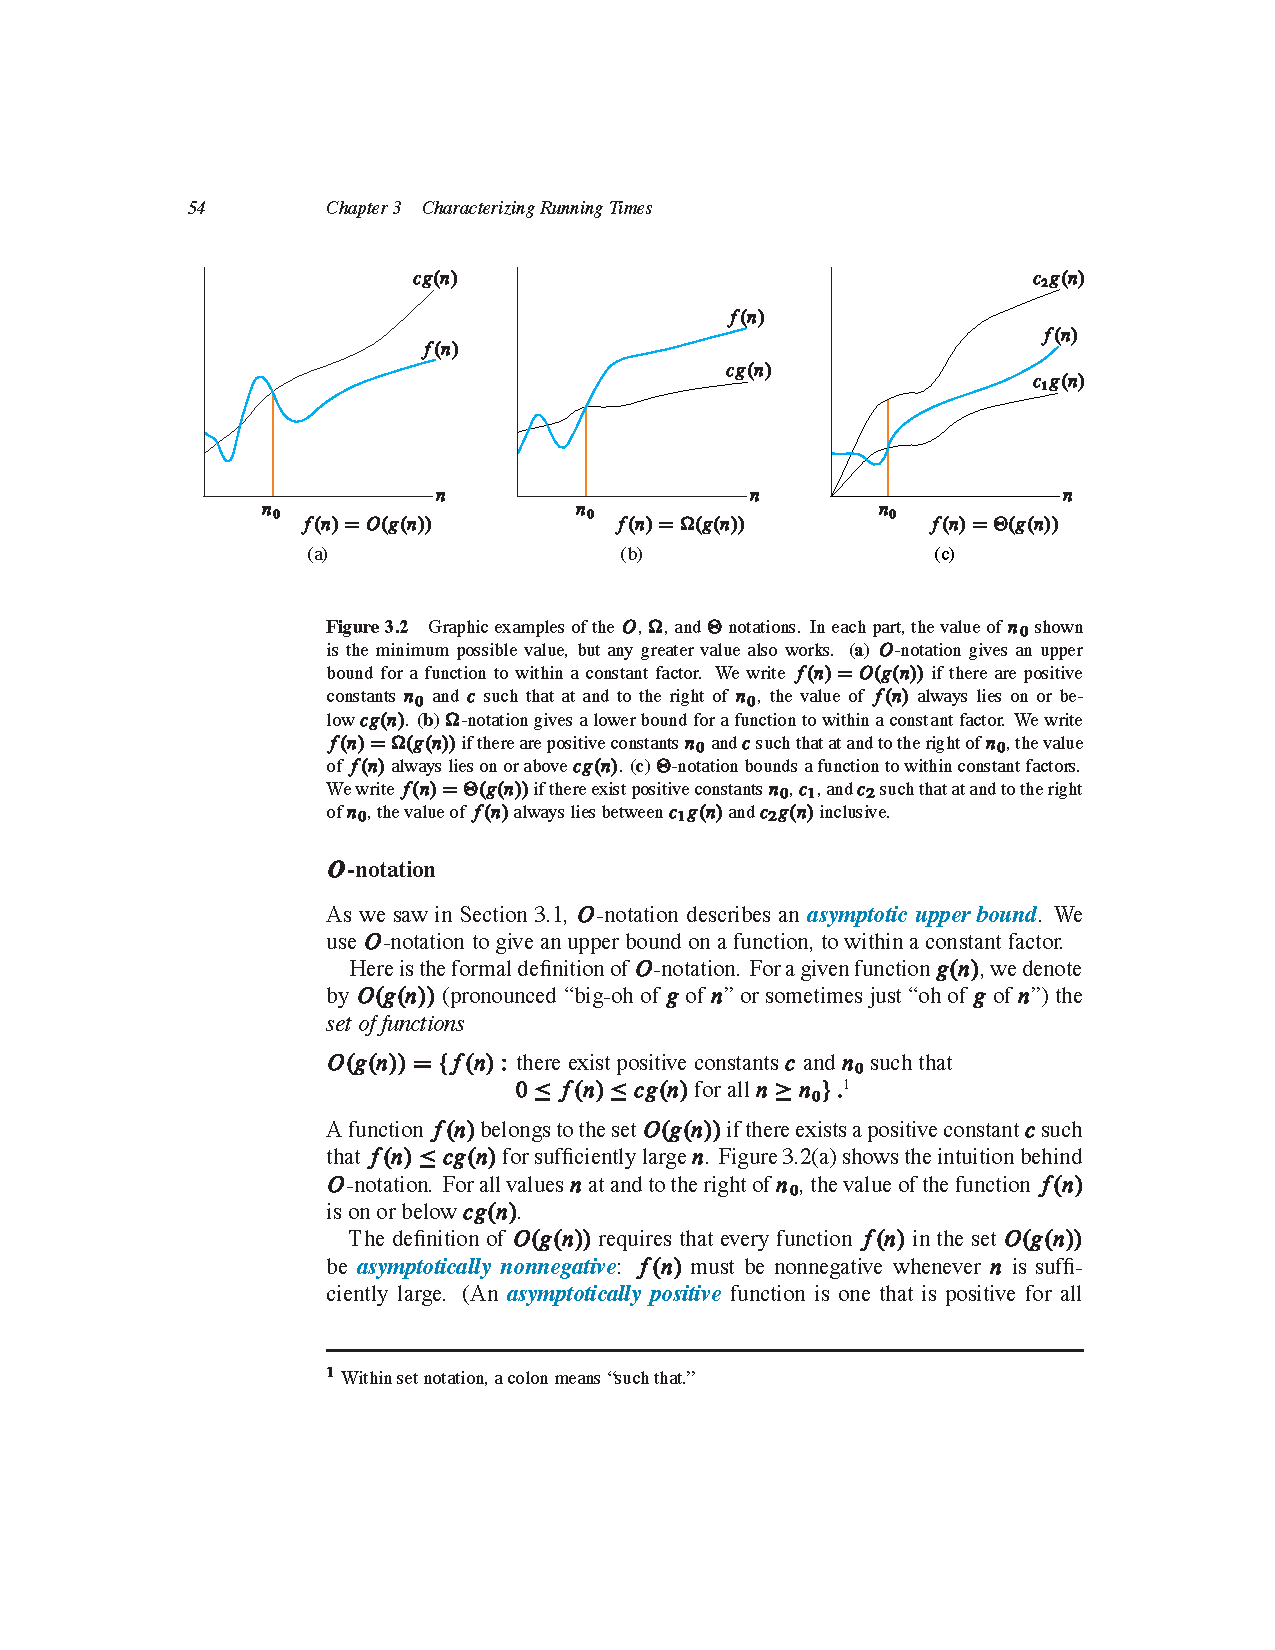
\includegraphics[width=0.4\textwidth, trim={3.25cm 18.75cm 13.85cm 4.60cm}, clip]{figures/bigs}
\end{frame}

\begin{frame}{$O$-notation (upper bounds)}
    \begin{tcolorbox}
        \vspace{-3mm}
        \begin{align*}
            O(g(n)) = \{ f(n):  & \text{ there exist constants } \\
                                                   & c > 0, n_0 > 0 \text{ such that } \\
                                                   & 0 \leq f(n) \leq cg(n) \\
                                                   & \text{for all } n \geq n_0\}
        \end{align*}
    \end{tcolorbox}
    \begin{block}{Example}
        $2n^2 = O(n^3) \hspace{10mm} (c = 1, n_0 = 2).$
    \end{block}
\end{frame}

\begin{frame}{$O$-notation (upper bounds)}
    \begin{tcolorbox}
        \vspace{-3mm}
        \begin{align*}
            O(g(n)) = \{ f(n):  & \text{ there exist constants } \\
                                                   & c > 0, n_0 > 0 \text{ such that } \\
                                                   & 0 \leq f(n) \leq cg(n) \\
                                                   & \text{for all } n \geq n_0\}
        \end{align*}
    \end{tcolorbox}
    \begin{block}{Example}
        $2n^2 = O(n^3) \hspace{10mm} (c = 1, n_0 = 2).$
    \end{block}
    \vspace{10mm}
    Functions, \\not values!
    \begin{tikzpicture}[remember picture,overlay]   %% use here too
        \draw[red,thick,->] (-0.27, 0.57) to [out=0,in=270] (-0.30, 2.00);
        \draw[blue,thick,->] (-2.00, 0.10) to [out=150,in=270] (-1.70, 2.00);
    \end{tikzpicture}    
\end{frame}

\begin{frame}{$O$-notation (upper bounds)}
    \begin{tcolorbox}
        \vspace{-3mm}
        \begin{align*}
            O(g(n)) = \{ f(n):  & \text{ there exist constants } \\
                                                   & c > 0, n_0 > 0 \text{ such that } \\
                                                   & 0 \leq f(n) \leq cg(n) \\
                                                   & \text{for all } n \geq n_0\}
        \end{align*}
    \end{tcolorbox}
    \begin{block}{Example}
        $2n^2 = O(n^3) \hspace{10mm} (c = 1, n_0 = 2).$
    \end{block}
    \vspace{10mm}
    Functions, \\not values! 
    \begin{tikzpicture}[remember picture,overlay]   %% use here too
        \draw[red,thick,->] (-0.27, 0.57) to [out=0,in=270] (-0.30, 2.00);
        \draw[blue,thick,->] (-2.00, 0.10) to [out=150,in=270] (-1.70, 2.00);
        \draw[orange,thick,->] (2.00, 0.10) to [out=150,in=270] (-1.125, 2.00);
        \node[] at (4.40, 0.10) {\normalsize Funny, ``one-way'' equality...};
    \end{tikzpicture}    
\end{frame}

\begin{frame}{Set Definition of $O$-notation}
    \begin{tcolorbox}
        \begin{align*}
            O(g(n)) = \{ f(n): & \text{ there exist constants } \\
                                        & c > 0, n_0 > 0 \text{ such that } \\
                                        & 0 \leq f(n) \leq  cg(n) \\
                                        & \text{for all } n \geq n_0\}
        \end{align*}
    \end{tcolorbox}
\end{frame}

\begin{frame}{Set Definition of $O$-notation}
    \begin{tcolorbox}
        \begin{align*}
            O(g(n)) = \{ f(n): & \text{ there exist constants } \\
                                        & c > 0, n_0 > 0 \text{ such that } \\
                                        & 0 \leq f(n) \leq  cg(n) \\
                                        & \text{for all } n \geq n_0\}
        \end{align*}
    \end{tcolorbox}
    \begin{block}{Example:}
        $2n^2 \in O(n^3)$
    \end{block}
    \vspace{5mm}
    (\textit{Logicians:} $\lambda n.2n^2 \in O(\lambda n.n^3) $, but it's convenient to be sloppy, as long as we understand what's really going on.)
\end{frame}

\begin{frame}{Macro substitution}
    \begin{alertblock}{\textbf{Convention:}}
        A set in a formula represents an anonymous function in the set.
    \end{alertblock}
    \begin{exampleblock}{\textbf{Example:}}
        \vspace{2mm}
        $ f(n) = n^3 + O(n^2) $\\
        means \\
        $ f(n) = n^3 + h(n) $\\
        for some $h(n) \in O(n^2)$.
    \end{exampleblock}
\end{frame}

\begin{frame}{Macro substitution}
    \begin{alertblock}{\textbf{Convention:}}
        A set in a formula represents an anonymous function in the set.
    \end{alertblock}
    \begin{exampleblock}{\textbf{Example:}}
        \vspace{2mm}
        $ n^2 + O(n) = O(n^2) $\\
        means \\
        for any $ f(n) \in O(n)$:\\
        \hspace{6mm} $n^2 + f(n) = h(n)$\\
        \hspace{6mm} for some $h(n) \in O(n^2)$.
    \end{exampleblock}
\end{frame}

\begin{frame}{$\Omega$-notation (lower bounds)}
    \begin{tcolorbox}
        $O$-notation is an upper-bound notation.  It makes no sense to say $f(n)$ is at least $O(n^2)$
    \end{tcolorbox}
\end{frame}

\begin{frame}{$\Omega$-notation (lower bounds)}
    \begin{tcolorbox}
        \vspace{-3mm}
        \begin{align*}
            \Omega(g(n)) = \{ f(n):  & \text{ there exist constants } \\
                                                   & c > 0, n_0 > 0 \text{ such that } \\
                                                   & 0 \leq cg(n) \leq f(n) \\
                                                   & \text{for all } n \geq n_0\}
        \end{align*}
    \end{tcolorbox}
    \vspace{3mm}
    \centering
    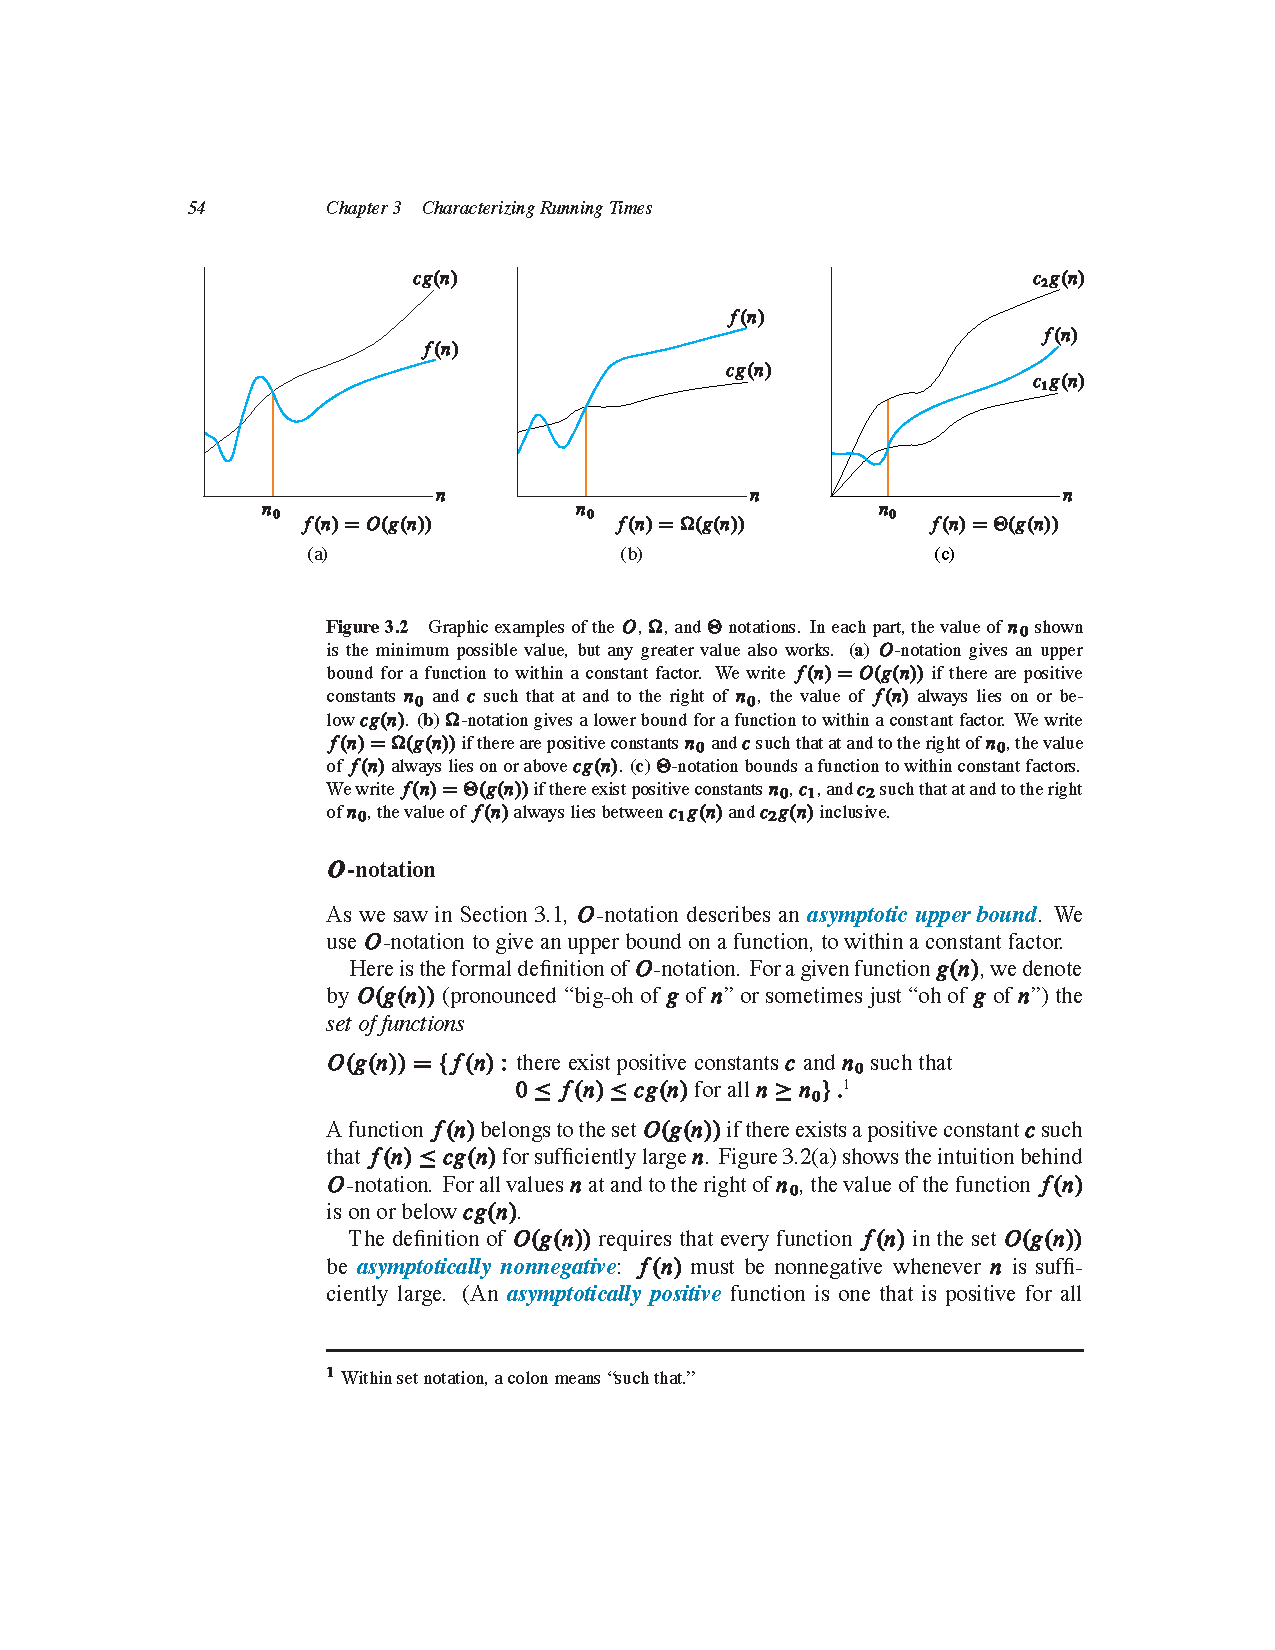
\includegraphics[width=0.4\textwidth, trim={8.30cm 18.75cm 8.30cm 4.60cm}, clip]{figures/bigs}
\end{frame}

\begin{frame}{$\Omega$-notation (lower bounds)}
    \begin{block}{}
        $O$-notation is an upper-bound notation.  It makes no sense to say $f(n)$ is at least $O(n^2)$
    \end{block}
    \begin{tcolorbox}
        \begin{align*}
            \Omega(g(n)) = \{ f(n):  & \text{ there exist constants } \\
                                                   & c > 0, n_0 > 0 \text{ such that } \\
                                                   & 0 \leq cg(n) \leq f(n) \\
                                                   & \text{for all } n \geq n_0\}
        \end{align*}
    \end{tcolorbox}
    \begin{exampleblock}{\textbf{Example:}}
        \vspace{2mm}
        $ \sqrt{n} = \Omega(\lg n) $ \hspace{5mm} $(c = 1, n_0 = 16)$ \\
    \end{exampleblock}
\end{frame}

\begin{frame}{$\Theta$-notation (tight bounds)}
    \begin{tcolorbox}
        $\Theta(g(n)) = O(g(n)) \cap \Omega(g(n))$
    \end{tcolorbox}
    \vspace{5mm}
    \centering
    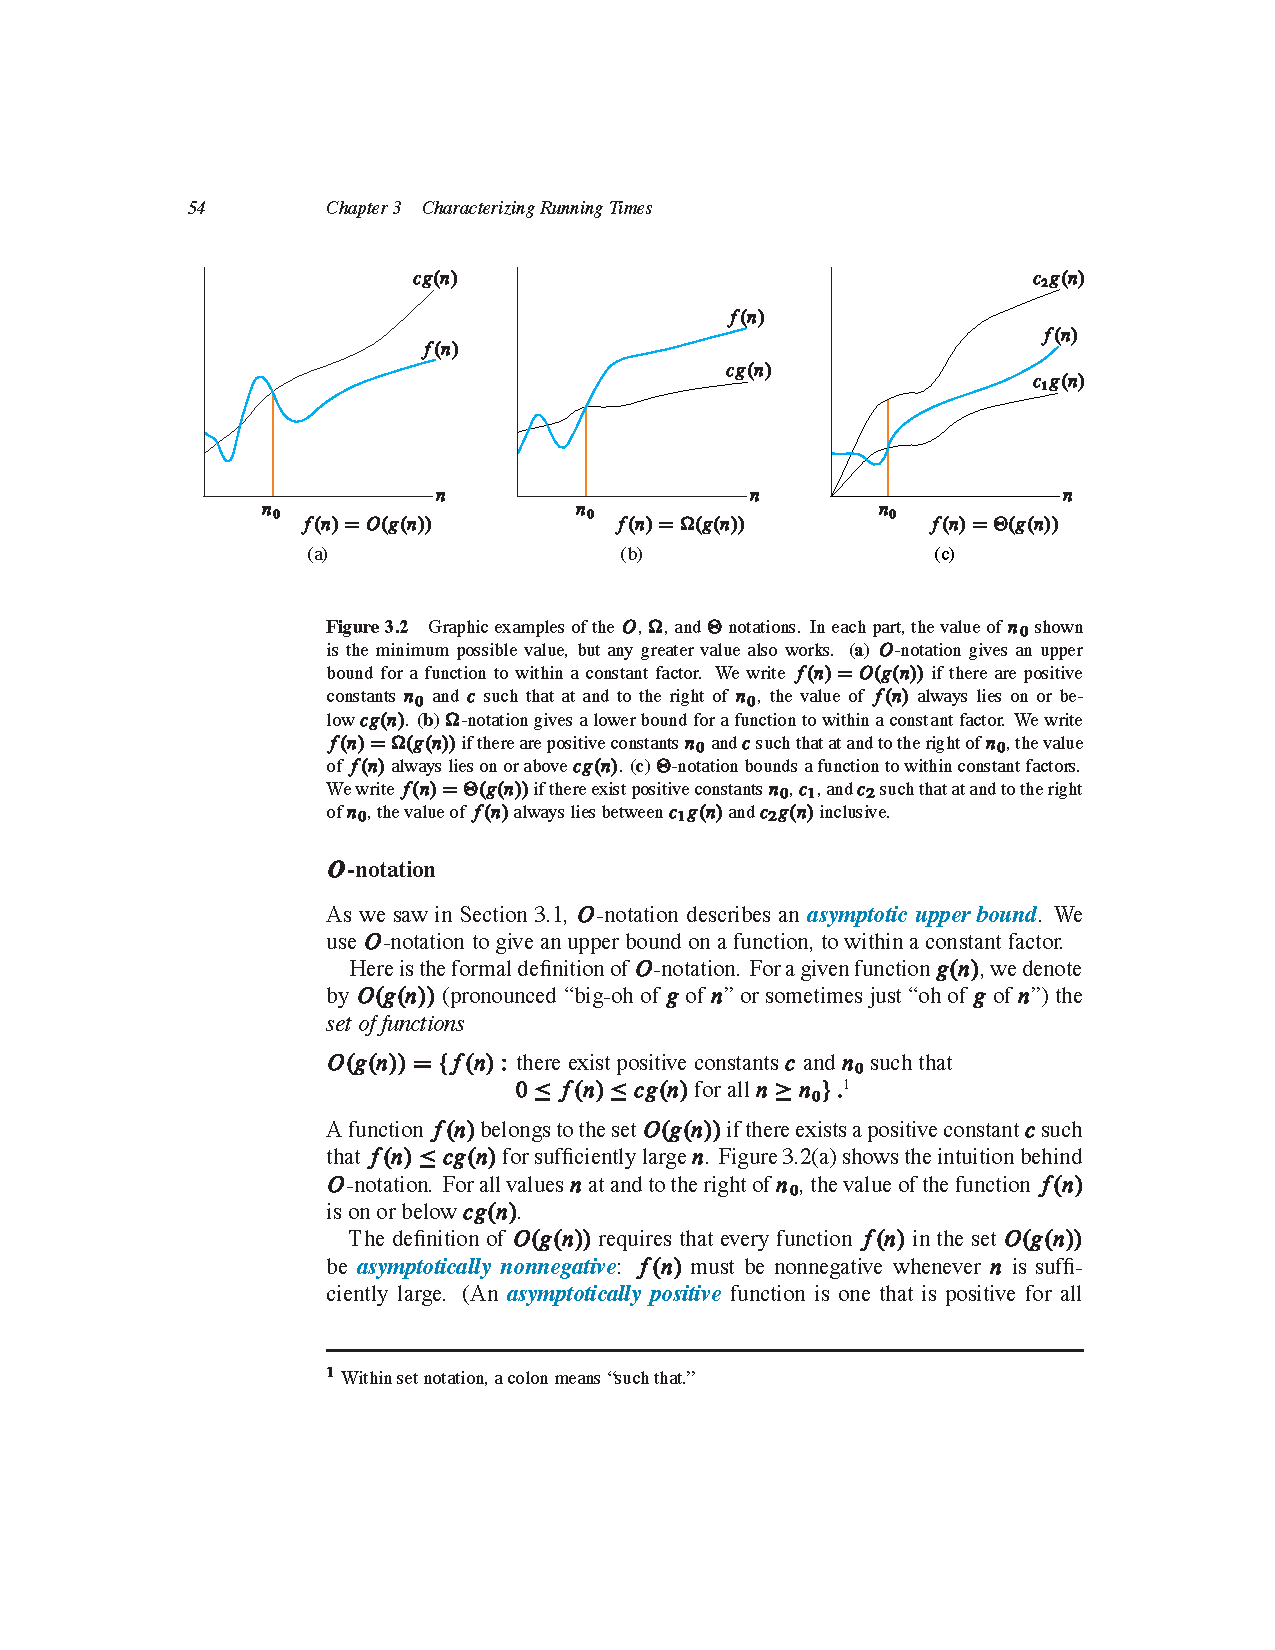
\includegraphics[width=0.4\textwidth, trim={13.90cm 18.75cm 3.23cm 4.60cm}, clip]{figures/bigs}
\end{frame}

\begin{frame}{$\Theta$-notation (tight bounds)}
    \begin{tcolorbox}
        $\Theta(g(n)) = O(g(n)) \cap \Omega(g(n))$
    \end{tcolorbox}
    \begin{exampleblock}{\textbf{Example:}}
        \vspace{2mm}
        $ \frac{1}{2}n^2 - 2n = \Theta(n^2) $
    \end{exampleblock}
\end{frame}

\begin{frame}{$o$-notation and $\omega$-notation}
    \begin{block}{}
        $O$-notation and $\Omega$-notation are like $\leq$ and $\geq$.\\
        $o$-notation and $\omega$-notation are like $<$ and $>$.
    \end{block}
    \begin{tcolorbox}
        \begin{align*}
            o(g(n)) = \{ f(n):  & \text{ for any constant } c > 0, \\
                                                   & \text{ there is a constant } n_0 > 0 \\
                                                   & \text{ such that } 0 \leq f(n) \leq cg(n) \\
                                                   & \text{ for all } n \geq n_0\}
        \end{align*}
    \end{tcolorbox}
    \begin{exampleblock}{\textbf{Example:}}
        \vspace{2mm}
        $ 2n^2 = o(n^3) $ \hspace{5mm} $(n_0 = \frac{2}{c})$
    \end{exampleblock}
\end{frame}

\begin{frame}{$o$-notation and $\omega$-notation}
    \begin{block}{}
        $O$-notation and $\Omega$-notation are like $\leq$ and $\geq$.\\
        $o$-notation and $\omega$-notation are like $<$ and $>$.
    \end{block}
    \begin{tcolorbox}
        \begin{align*}
            \omega(g(n)) = \{ f(n):  & \text{ for any constant } c > 0, \\
                                                   & \text{ there is a constant } n_0 > 0 \\
                                                   & \text{ such that } 0 \leq cg(n) \leq f(n) \\
                                                   & \text{ for all } n \geq n_0\}
        \end{align*}
    \end{tcolorbox}
    \begin{exampleblock}{\textbf{Example:}}
        \vspace{2mm}
        $ \sqrt{n} = \omega(\lg n) $ \hspace{5mm} $(n_0 = 1 + \frac{1}{c})$
    \end{exampleblock}
\end{frame}

\section{Solving recurrences}

\begin{frame}{Solving recurrences}
    \begin{itemize}
        \item The analysis of merge-sort from \textbf{\textit{Lecture 1}} required us to solve a recurrence.
        \item Recurrences are like solving integrals, differential equations, etc.
        \begin{itemize}
            \item Learn a few tricks.
        \end{itemize}
        \item \textbf{\textit{Lecture 3:}} Applications of recurrences to divide-and-conquer algorithms.
    \end{itemize}
\end{frame}

\subsection{Substitution method}

\begin{frame}{Substitution method}
    The method is based on guessing a possible solution and then verifying it using mathematical induction. It is divided into the following steps:
    \begin{enumerate}
        \item \textbf{Guess a solution:} Propose a general form of the solution $T(n)$, based on the structure of the problem.
        \item \textbf{Substitute into the recurrence:} Replace the conjectured solution in the recurrence equation to check if it holds.
        \item \textbf{Adjust if necessary:} If the conjecture is not valid, modify it by adding constants or additional terms.
        \item \textbf{Prove by induction:} Use mathematical induction to demonstrate that the conjecture is correct.
    \end{enumerate}
\end{frame}

\begin{frame}{Substitution method}
    The most general method:
    \begin{enumerate}
        \item \textbf{Guess} the form of the solution.
        \item \textbf{Verify} by induction.
        \item \textbf{Solve} for constants.
    \end{enumerate}
\end{frame}

\begin{frame}{Substitution method}
    The most general method:
    \begin{enumerate}
        \item \textbf{Guess} the form of the solution.
        \item \textbf{Verify} by induction.
        \item \textbf{Solve} for constants.
    \end{enumerate}
    \begin{exampleblock}{\textbf{Example:}}
        \vspace{2mm}
        $ T(n) = 4T(\frac{n}{2}) + n$
        \begin{itemize}
            \item Assume that $T(1) = \Theta(1)$.
            \item Guess $O(n^3)$. \textit{(Prove $O$ and $\Omega$ separately.)}
            \item Assume that $T(k) \leq ck^3$ for $k < n$.
            \item Prove $T(n) \leq cn^3$ by induction.
        \end{itemize}
    \end{exampleblock}
\end{frame}

\begin{frame}{Example of substitution}
    \begin{align*}
        T(n) = & \text{ }4T \left(\frac{n}{2}\right) + n \\
            \leq & \text{ }4c \left(\frac{n}{2}\right)^3 + n \\
                = & \text{ }\left(\frac{c}{2}\right)n^3 + n \\
                = & \text{ }cn^3 - \left(\left(\frac{c}{2}\right)n^3 - n\right) \longleftarrow \text{ \textbf{desired} } - \text{ \textbf{residual} } \\
             \leq & \text{ }cn^3 \longleftarrow \text{ \textbf{desired} } \\
        \text{whenever }& \left(\frac{c}{2}\right)n^3 - n \geq 0\text{, for example, if } c \geq 2 \text{ and } n \geq 1\text{.} 
    \end{align*}
    \begin{tikzpicture}[remember picture,overlay]   %% use here too
        \draw[orange,thick,->] (6.00, -0.40) to [out=90,in=270] (3.55, 0.85);
        \node[] at (6.40, -0.50) {\normalsize \textbf{residual}};
    \end{tikzpicture}    
\end{frame}

\begin{frame}{Example (continued)}
    \begin{itemize}
        \item We must also handle the initial conditions, that is, ground the induction with base cases.
        \item \textbf{Base:} $T(n) = \Theta(1)$ for all $n \leq n_0$, where $n_0$ is a suitable constant.
        \item For $1 \leq n < n_0$, we have ``$\Theta(1)$'' $\leq cn^3$, if we pick $c$ big enough.
    \end{itemize}
\end{frame}

\begin{frame}{Example (continued)}
    \begin{itemize}
        \item We must also handle the initial conditions, that is, ground the induction with base cases.
        \item \textbf{Base:} $T(n) = \Theta(1)$ for all $n \leq n_0$, where $n_0$ is a suitable constant.
        \item For $1 \leq n < n_0$, we have ``$\Theta(1)$'' $\leq cn^3$, if we pick $c$ big enough.
    \end{itemize}
    \par\noindent\rule{\textwidth}{0.4pt}\vspace{-4.35mm}
    \par\noindent\rule{\textwidth}{0.8pt}\vspace{-4.50mm}
    \par\noindent\rule{\textwidth}{0.4pt}
    \begin{center}
        \textbf{This bound is not tight!}
    \end{center}
\end{frame}

\begin{frame}{¿A tighter upper bound?}
    We shall prove that $T(n) = O(n^2)$.
\end{frame}

\begin{frame}{¿A tighter upper bound?}
    We shall prove that $T(n) = O(n^2)$.
    
    \begin{block}{}
        Assume that $T(k) \leq ck^2$ for $k < n$:
        \begin{align*}
            T(n) = & \text{ }4T \left(\frac{n}{2} \right) + n \\
                \leq & \text{ }4c \left(\frac{n}{2} \right)^2 + n \\
                   = & \text{ }cn^2 + n \\
                   = & \text{ }O(n^2) \\
        \end{align*}
    \end{block}
\end{frame}

\begin{frame}{¿A tighter upper bound?}
    We shall prove that $T(n) = O(n^2)$.
    
    \begin{block}{}
        Assume that $T(k) \leq ck^2$ for $k < n$:
        \begin{align*}
            T(n) = & \text{ }4T \left(\frac{n}{2} \right) + n \\
                \leq & \text{ }4c \left(\frac{n}{2} \right)^2 + n \\
                   = & \text{ }cn^2 + n \\
                   = & \text{ }O(n^2) \text{ \textbf{Wrong!} We must prove the I.H.}\\
        \end{align*}
    \end{block}
    \begin{tikzpicture}[remember picture,overlay]   %% use here too
        \draw[orange,thick,->] (9.00, 2.10) to [out=90,in=0] (6.00, 5.00);
        \draw (3.20, 1.75) node[cross, red, ultra thick] {};
    \end{tikzpicture}    
\end{frame}

\begin{frame}{¿A tighter upper bound?}
    We shall prove that $T(n) = O(n^2)$.
    
    \begin{block}{}
        Assume that $T(k) \leq ck^2$ for $k < n$:
        \begin{align*}
            T(n) = & \text{ }4T \left(\frac{n}{2} \right) + n \\
                \leq & \text{ }4c \left(\frac{n}{2} \right)^2 + n \\
                   = & \text{ }cn^2 + n \\
                   = & \text{ }O(n^2) \text{ \textbf{Wrong!} We must prove the I.H. }\\
                   = & \text{ }cn^2 -(-n) \text{ [ \textbf{desired} } - \text{ \textbf{residual} ] }\\
                 \leq& \text{ }cn^2 \text{    for \textbf{no} choice of } c > 0 \text{. Lose!}  
        \end{align*}
    \end{block}
    \begin{tikzpicture}[remember picture,overlay]   %% use here too
        \draw[orange,thick,->] (9.00, 2.70) to [out=90,in=0] (6.00, 5.70);
        \draw (3.20, 2.50) node[cross, red, ultra thick] {};
    \end{tikzpicture}    
\end{frame}

\begin{frame}{¡A tighter upper bound!}
    \begin{block}{\textsc{Idea}:}
        \begin{itemize}
        \item Strengthen the inductive hypothesis.
         \item \textbf{Subtract} a low-order term.
         \item \textit{Inductive hypothesis:} $T(k) \leq c_1k^2 - c_2k$ for $k < n$.
        \end{itemize}
    \end{block}
\end{frame}

\begin{frame}{¡A tighter upper bound!}
    \begin{block}{\textsc{Idea}:}
        \begin{itemize}
        \item Strengthen the inductive hypothesis.
         \item \textbf{Subtract} a low-order term.
         \item \textit{Inductive hypothesis:} $T(k) \leq c_1k^2 - c_2k$ for $k < n$.
        \end{itemize}
    \end{block}
    \begin{align*}
        T(n) = & \text{ }4T\left(\frac{n}{2}\right) + n \\
               = & \text{ }4\left(c_1\left(\frac{n}{2}\right)^2 - c_2\left(\frac{n}{2}\right)\right) + n \\
               = & \text{ }c_1n^2 - 2c_2n + n \\
               = & \text{ }c_1n^2 - c_2n - c_2n + n \\
               = & \text{ }c_1n^2 - c_2n - (c_2n - n) \\
               \leq & \text{ }c_1n^2 - c_2n \text{ if } c_2 \geq 1 \text{.} \\
    \end{align*}
\end{frame}

\begin{frame}{¡A tighter upper bound!}
    \begin{block}{\textsc{Idea}:}
        \begin{itemize}
        \item Strengthen the inductive hypothesis.
         \item \textbf{Subtract} a low-order term.
         \item \textit{Inductive hypothesis:} $T(k) \leq c_1k^2 - c_2k$ for $k < n$.
        \end{itemize}
    \end{block}
    \vspace{-5mm}
    \begin{align*}
        T(n) = & \text{ }4T\left(\frac{n}{2}\right) + n \\
               = & \text{ }4\left(c_1\left(\frac{n}{2}\right)^2 - c_1\left(\frac{n}{2}\right)\right) + n \\
               = & \text{ }c_1n^2 - 2c_2n + n \\
               = & \text{ }c_1n^2 - c_2n - c_2n + n \\
               = & \text{ }c_1n^2 - c_2n - (c_2n - n) \\
               \leq & \text{ }c_1n^2 - c_2n \text{ if } c_2 \geq 1 \text{.} \\
    \end{align*}
    \vspace{-15mm}
    \begin{block}{}
        Pick $c_1$ big enough to handle the initial conditions.
    \end{block}
\end{frame}

\subsection{Recursion tree}

\begin{frame}{Recursion-tree method}
    \begin{itemize}
        \item A recursion tree models the costs (time) of a recursive execution of an algorithm.
        \item The recursion-tree method can be unreliable, just like any method that uses ellipses $(\ldots)$.
        \item The recursion-tree method promotes intuition, however.
        \item The recursion-tree method is good for generating guesses for the substitution method.
    \end{itemize}
\end{frame}

\begin{frame}{Steps of the recurrence-tree method}
    \begin{enumerate}
        \item \textbf{Expand the recurrence} over multiple levels until a general pattern emerges.
        \item \textbf{Determine the cost at each level}, which usually depends on the number of subproblems and their size.
        \item \textbf{Calculate the depth of the tree}, which is the total number of levels until reaching base cases.
        \item \textbf{Sum the costs of all levels} to obtain the overall cost.
    \end{enumerate}
\end{frame}

\begin{frame}{Example of recursion tree}
    Solve $T(n) = T\left(\frac{n}{4}\right) + T\left(\frac{n}{2}\right) + n^2$
    \vspace{5.45cm}
\end{frame}

\begin{frame}{Example of recursion tree}
    Solve $T(n) = T\left(\frac{n}{4}\right) + T\left(\frac{n}{2}\right) + n^2$
    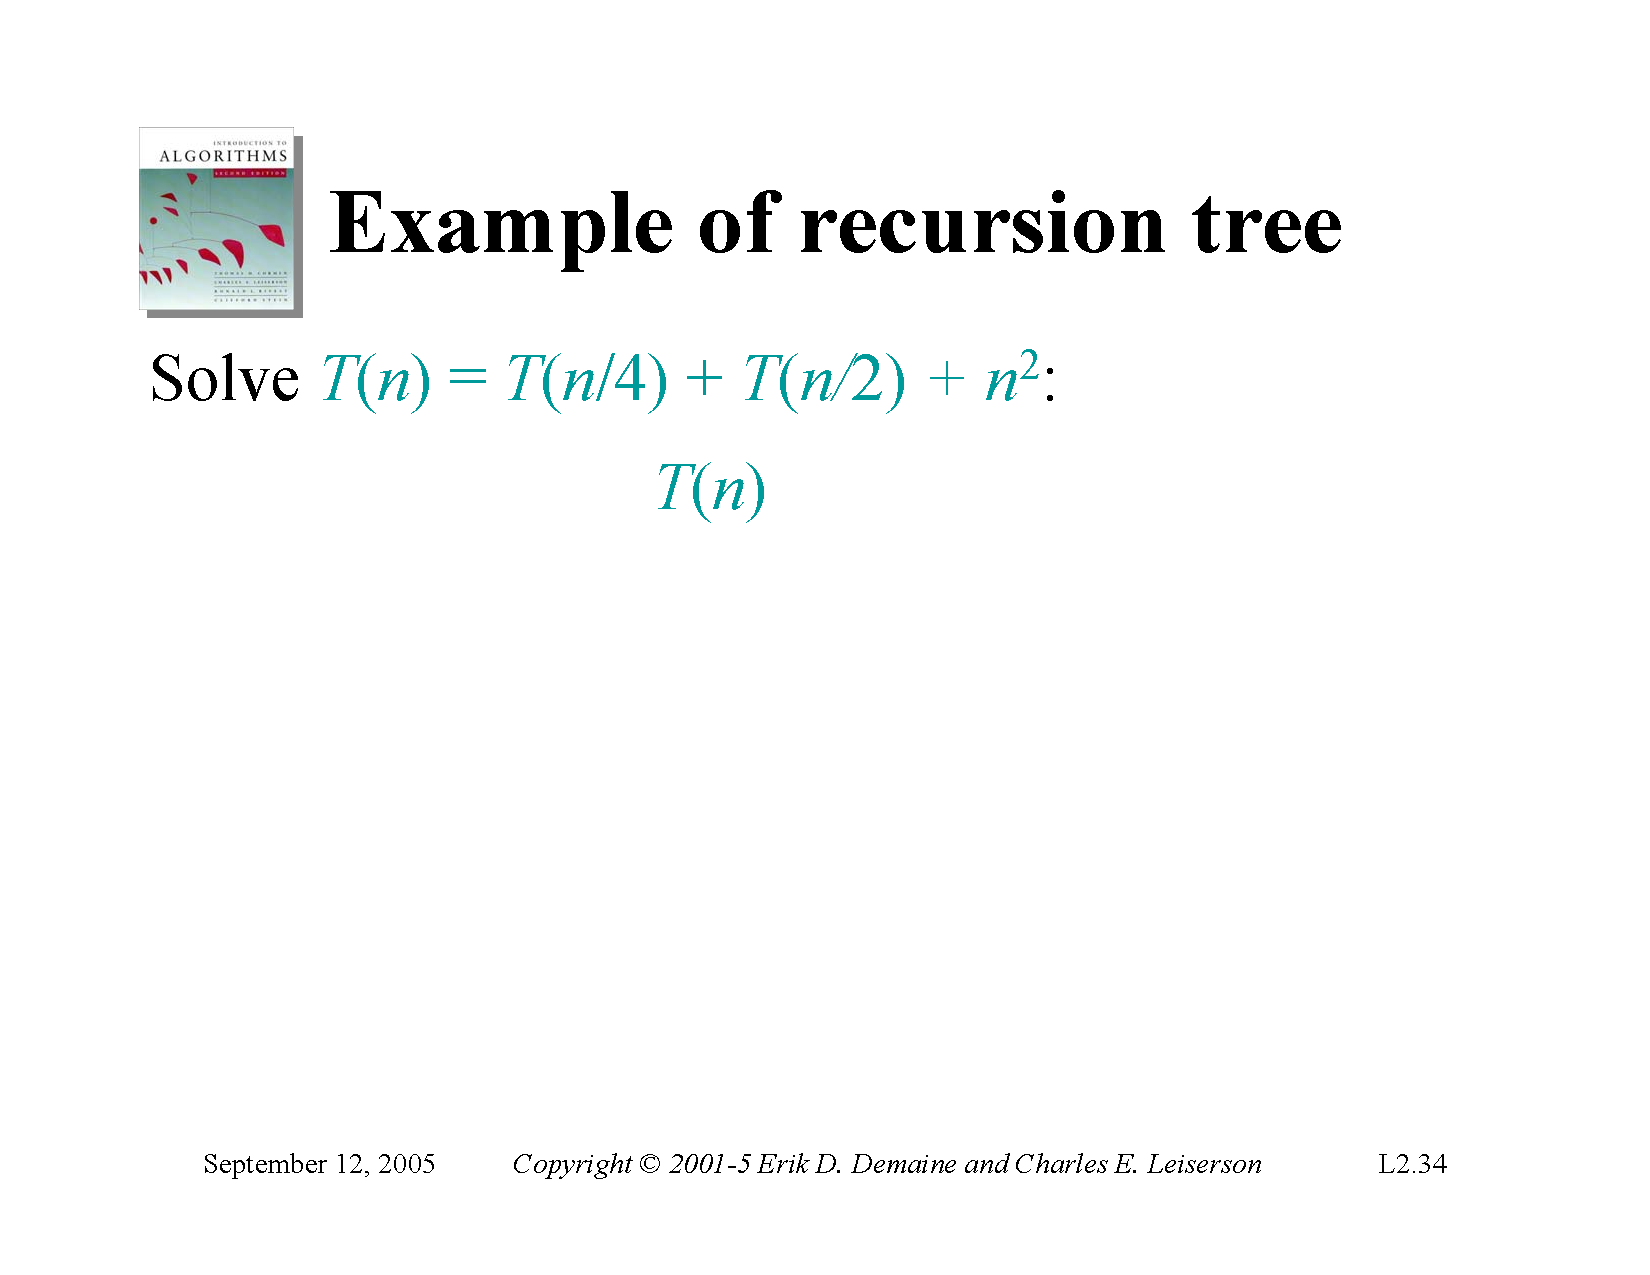
\includegraphics[width=\textwidth, trim={1.10cm 1.20cm 0.30cm 5.75cm}, clip]{pages/lec2_34}
\end{frame}
\begin{frame}{Example of recursion tree}
    Solve $T(n) = T\left(\frac{n}{4}\right) + T\left(\frac{n}{2}\right) + n^2$
    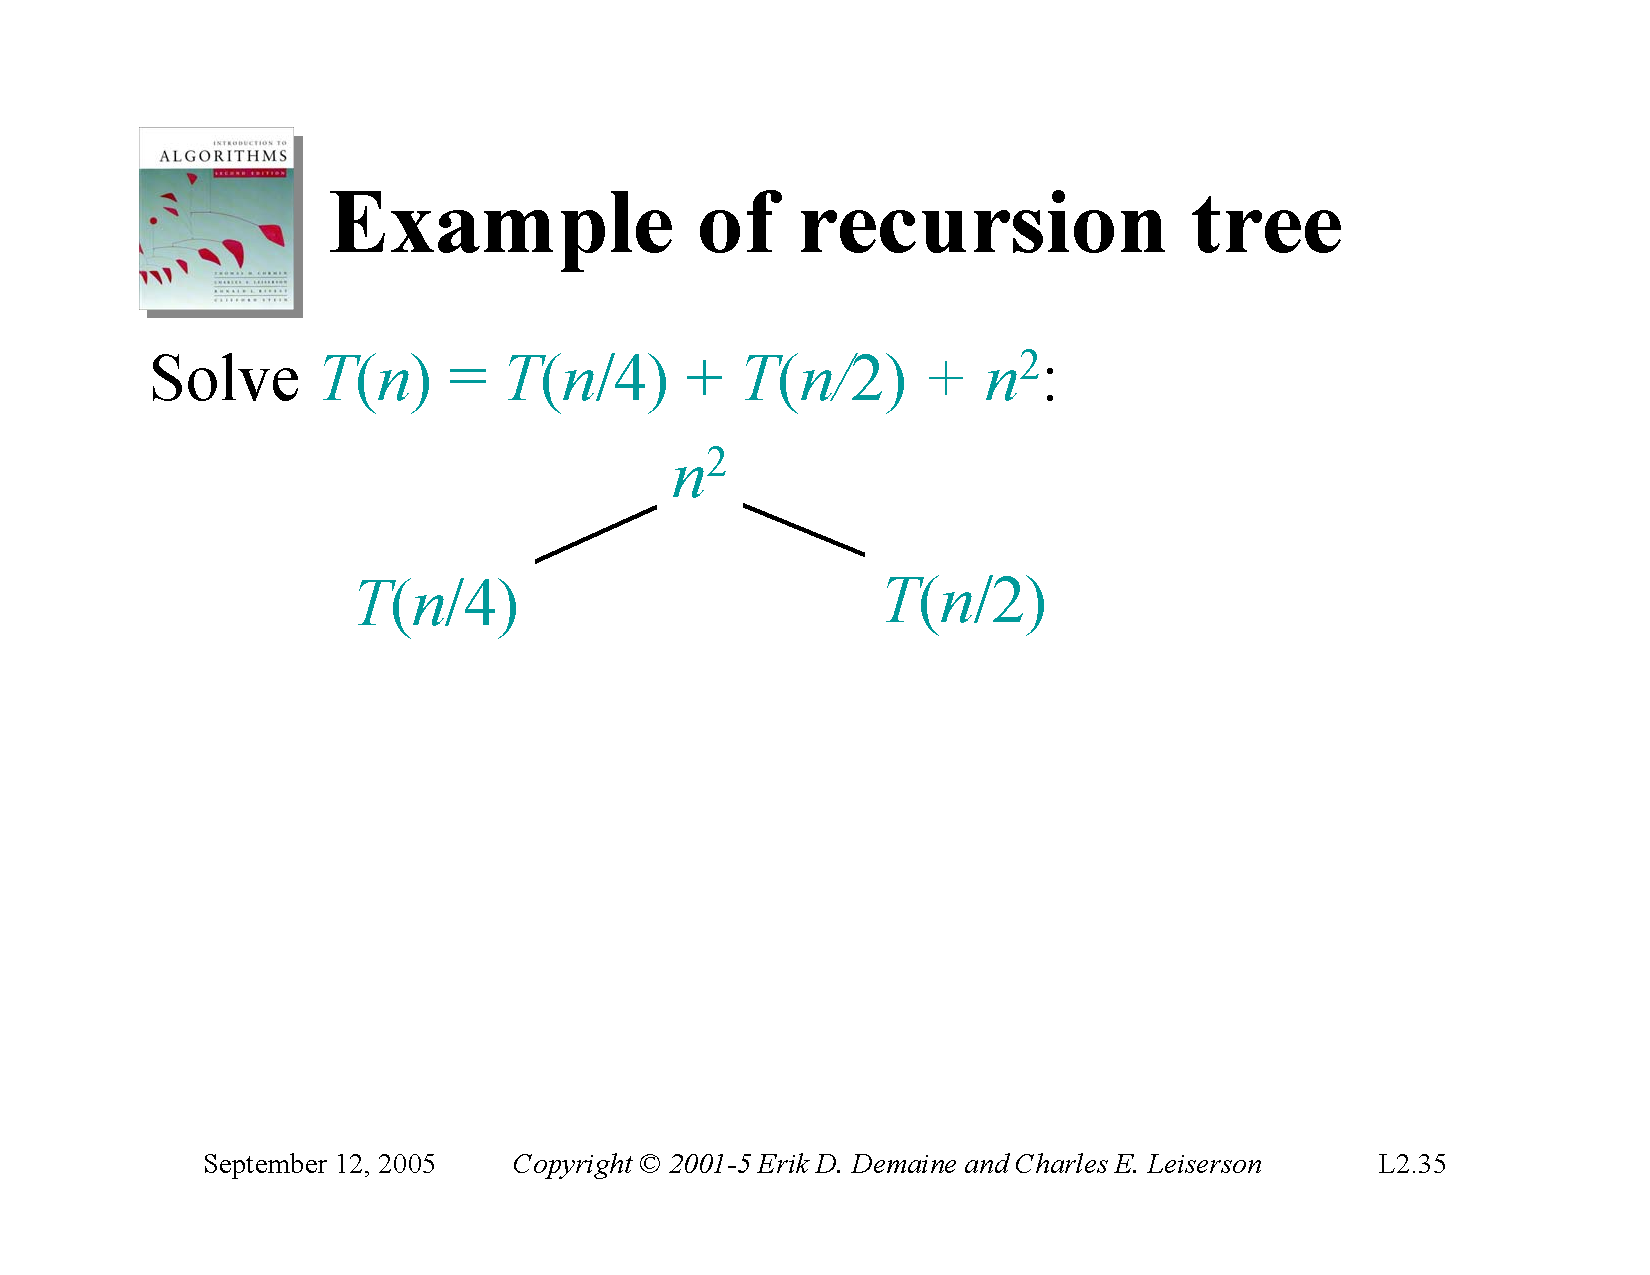
\includegraphics[width=\textwidth, trim={1.10cm 1.20cm 0.30cm 5.75cm}, clip]{pages/lec2_35}
\end{frame}
\begin{frame}{Example of recursion tree}
    Solve $T(n) = T\left(\frac{n}{4}\right) + T\left(\frac{n}{2}\right) + n^2$
    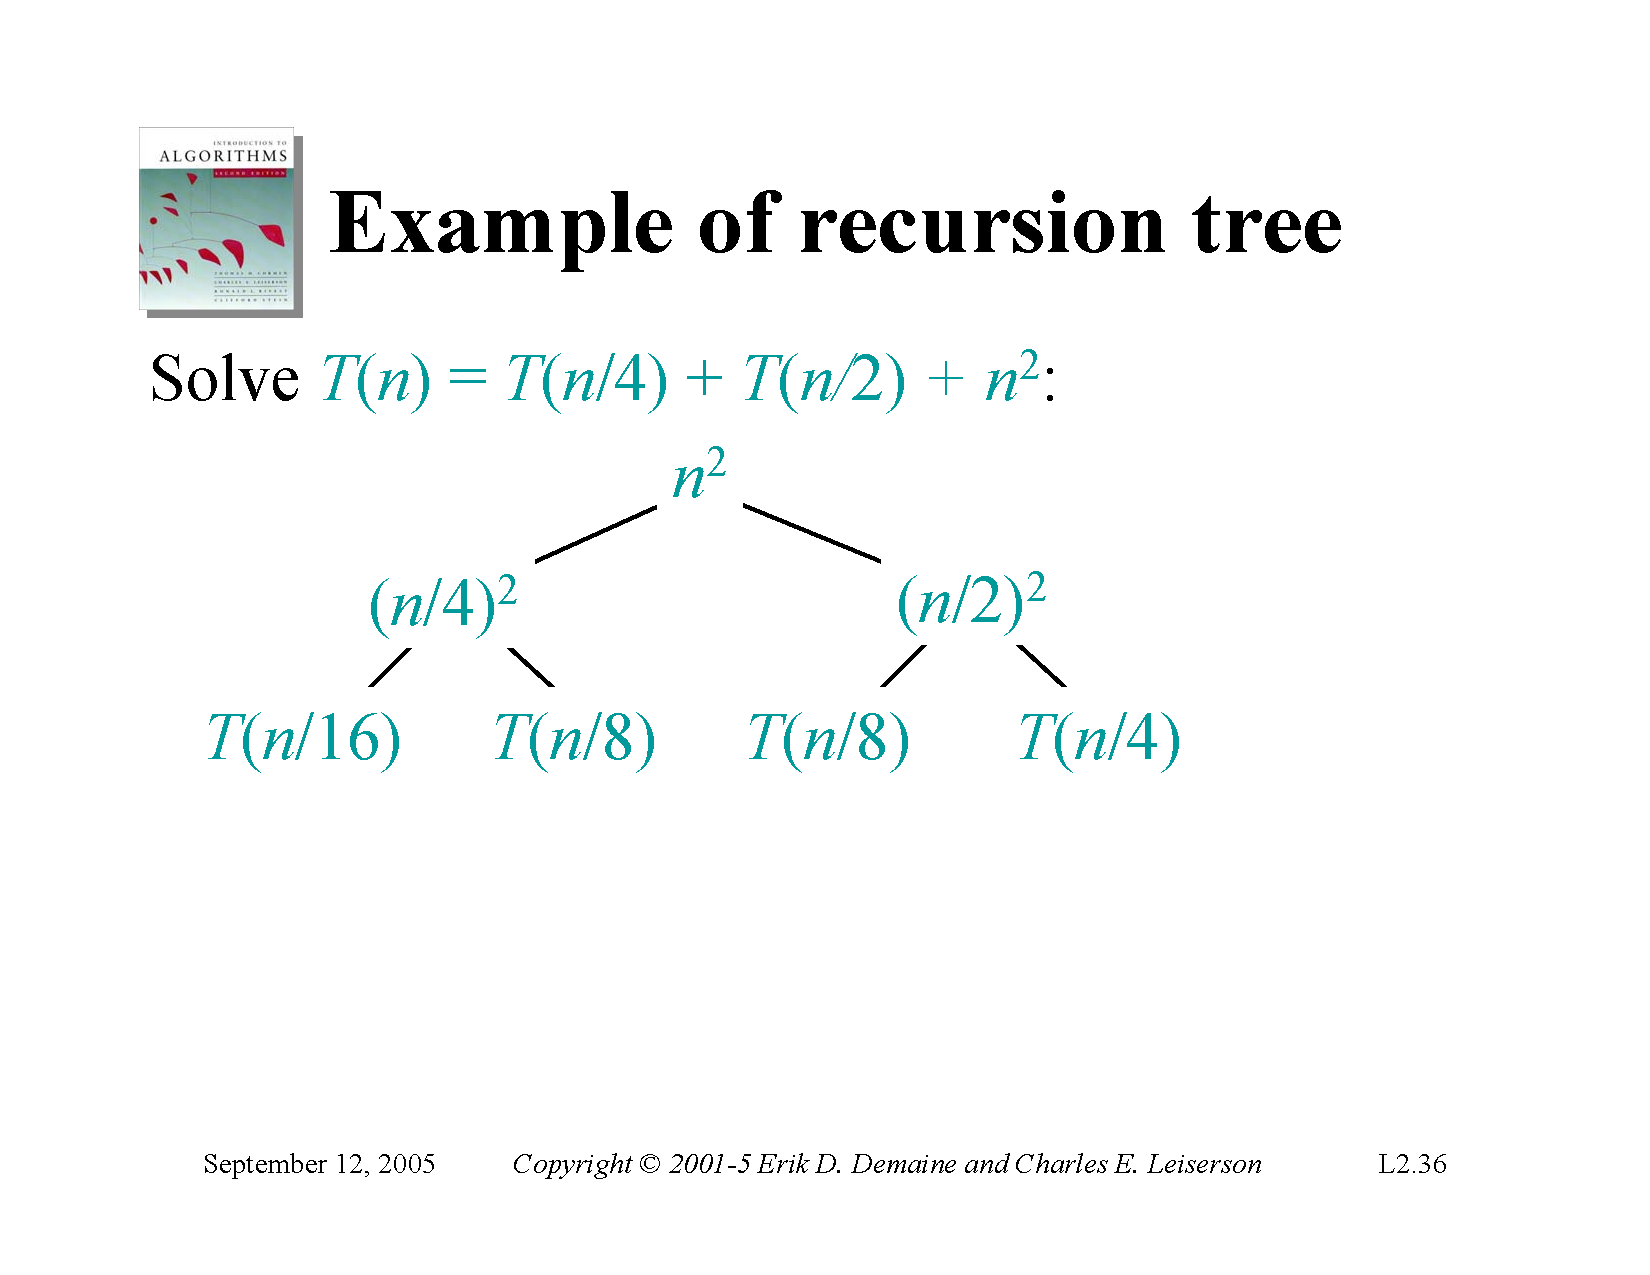
\includegraphics[width=\textwidth, trim={1.10cm 1.20cm 0.30cm 5.75cm}, clip]{pages/lec2_36}
\end{frame}
\begin{frame}{Example of recursion tree}
    Solve $T(n) = T\left(\frac{n}{4}\right) + T\left(\frac{n}{2}\right) + n^2$
    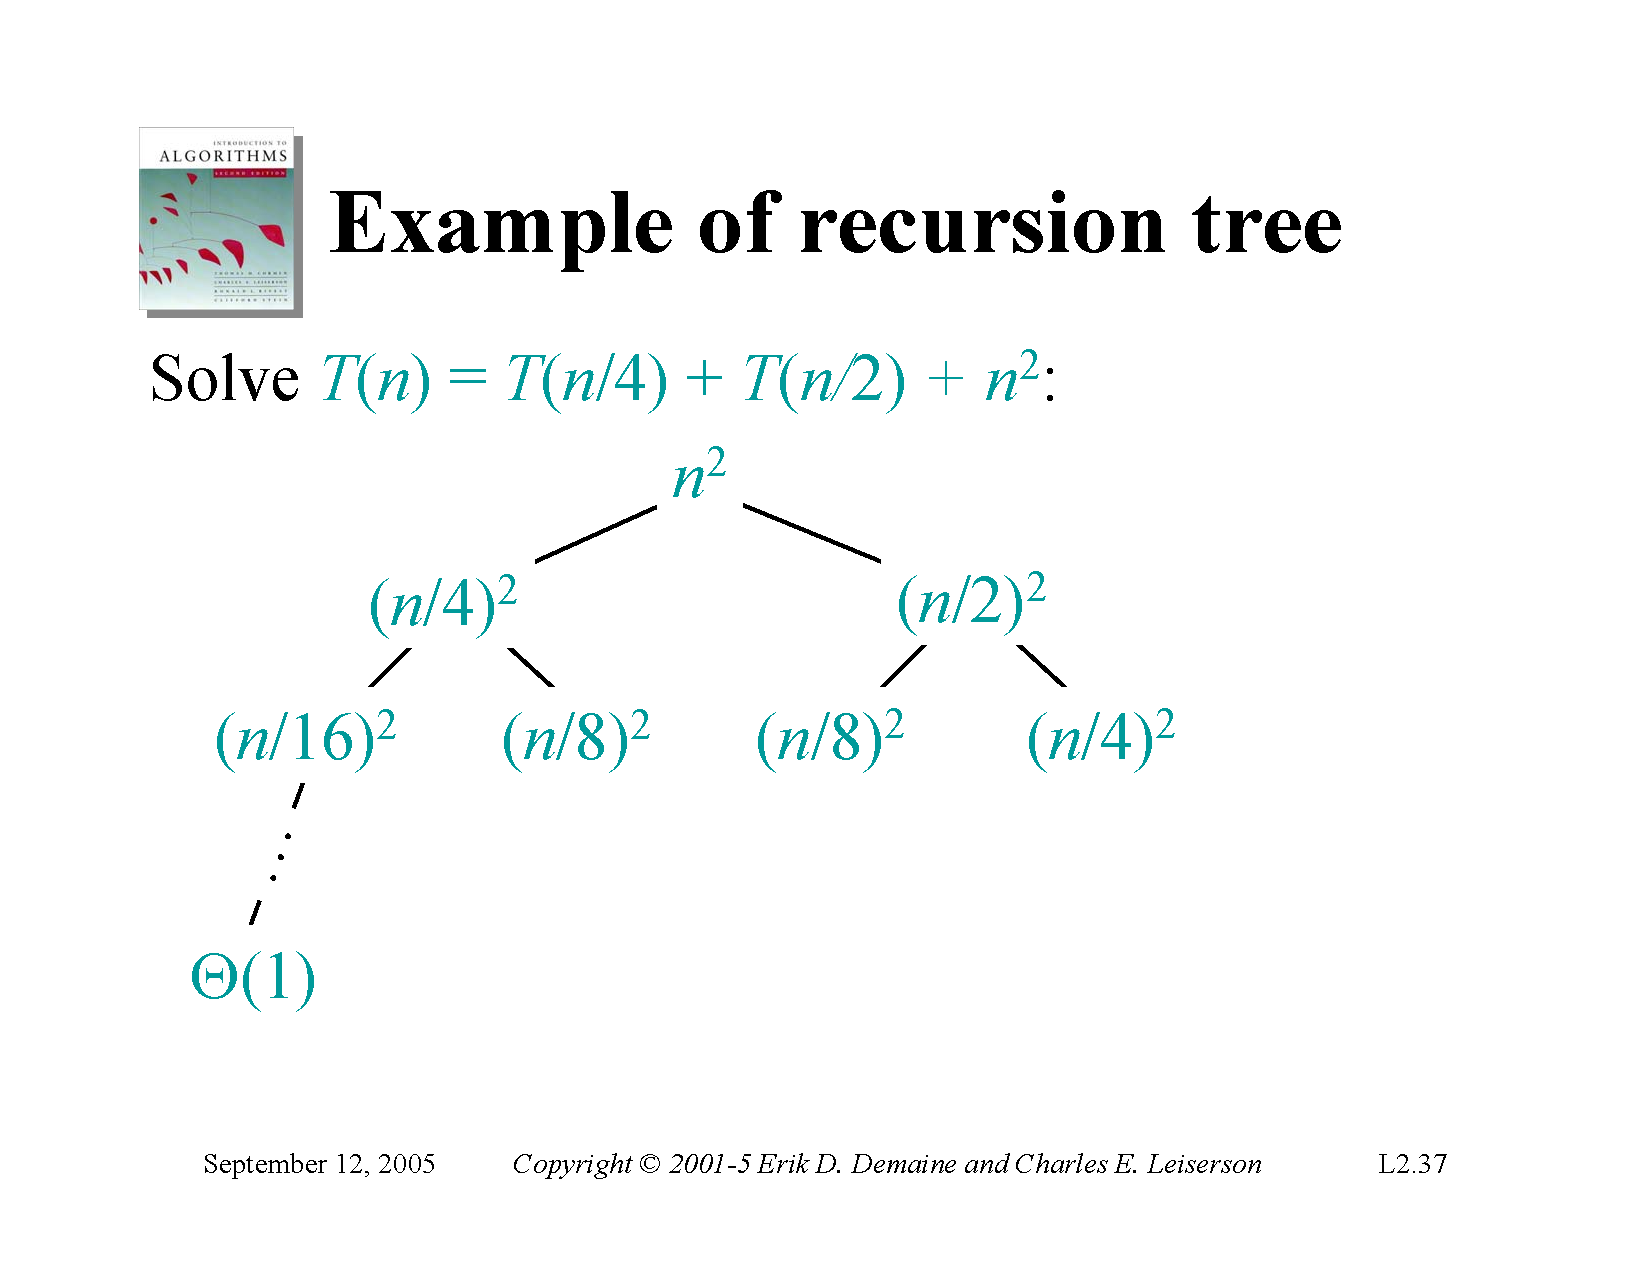
\includegraphics[width=\textwidth, trim={1.10cm 1.20cm 0.30cm 5.75cm}, clip]{pages/lec2_37}
\end{frame}
\begin{frame}{Example of recursion tree}
    Solve $T(n) = T\left(\frac{n}{4}\right) + T\left(\frac{n}{2}\right) + n^2$
    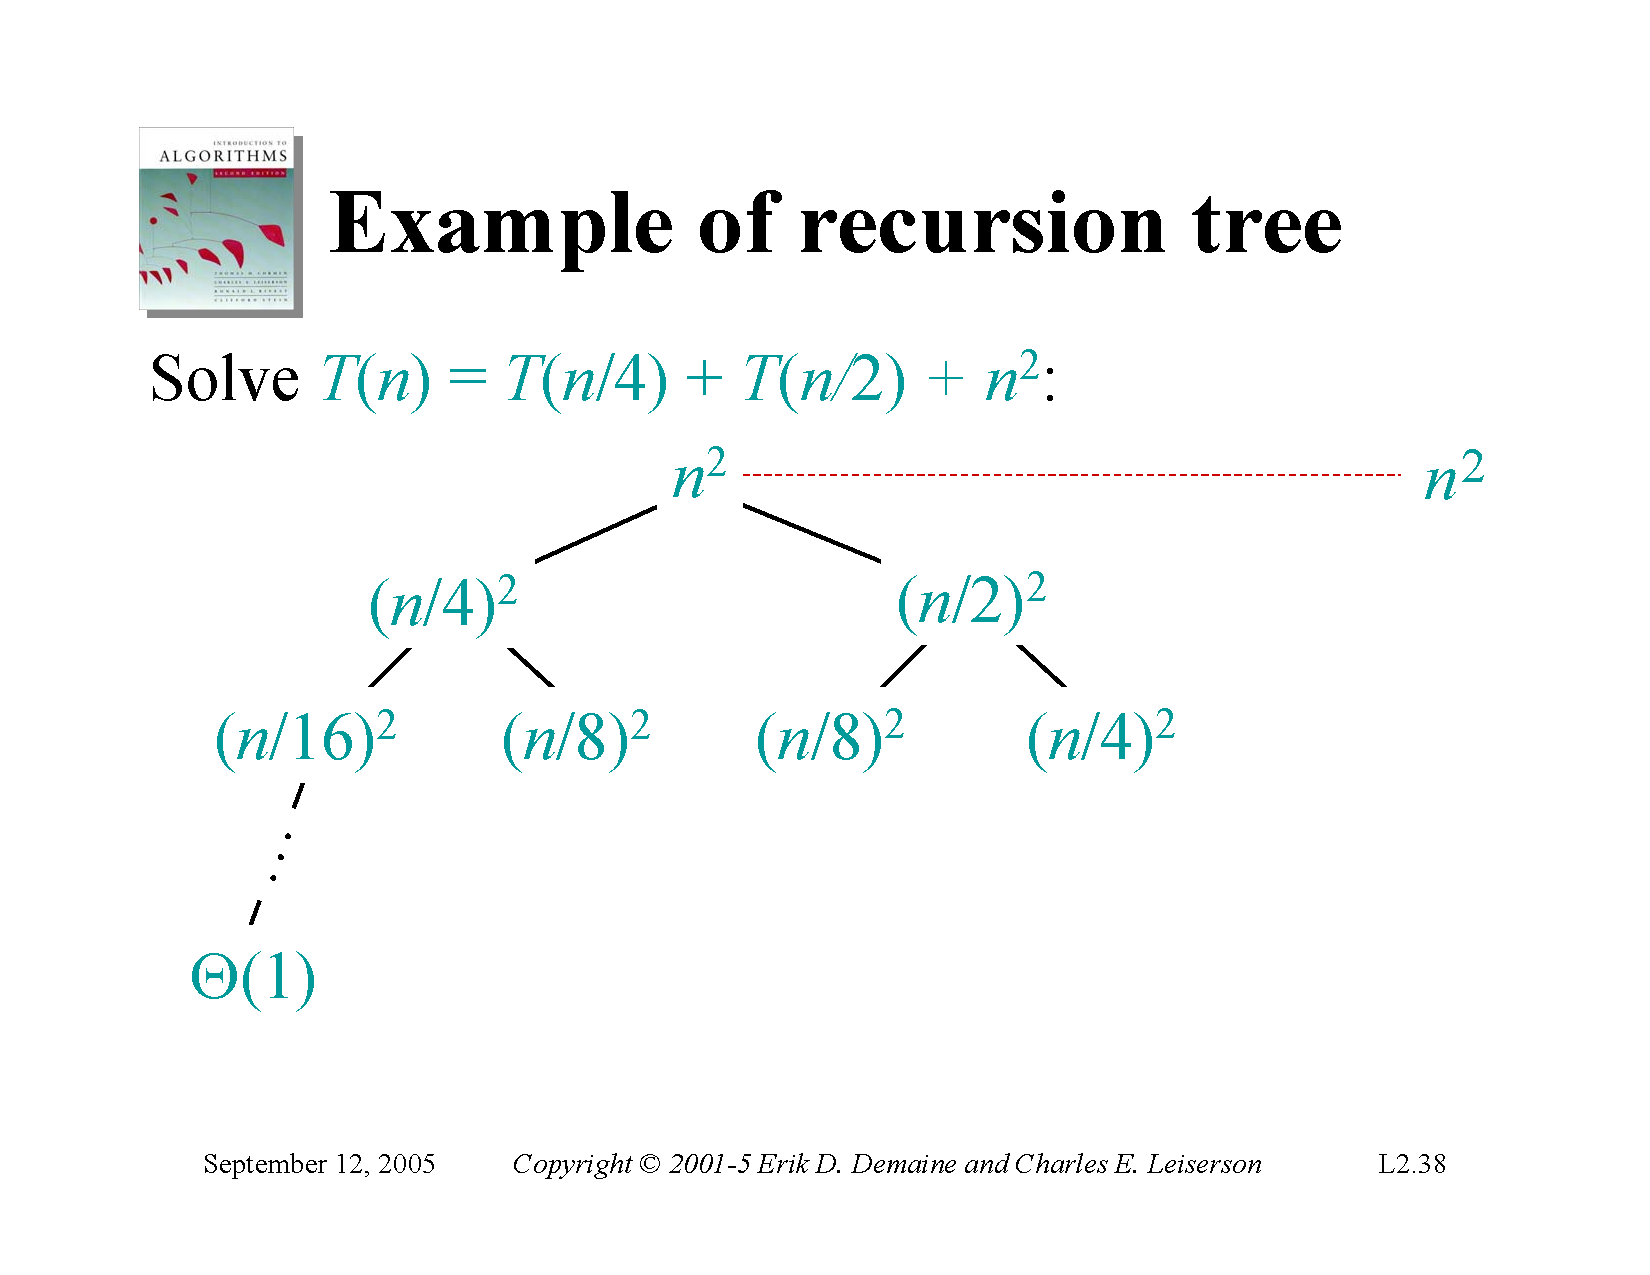
\includegraphics[width=\textwidth, trim={1.10cm 1.20cm 0.30cm 5.75cm}, clip]{pages/lec2_38}
\end{frame}
\begin{frame}{Example of recursion tree}
    Solve $T(n) = T\left(\frac{n}{4}\right) + T\left(\frac{n}{2}\right) + n^2$
    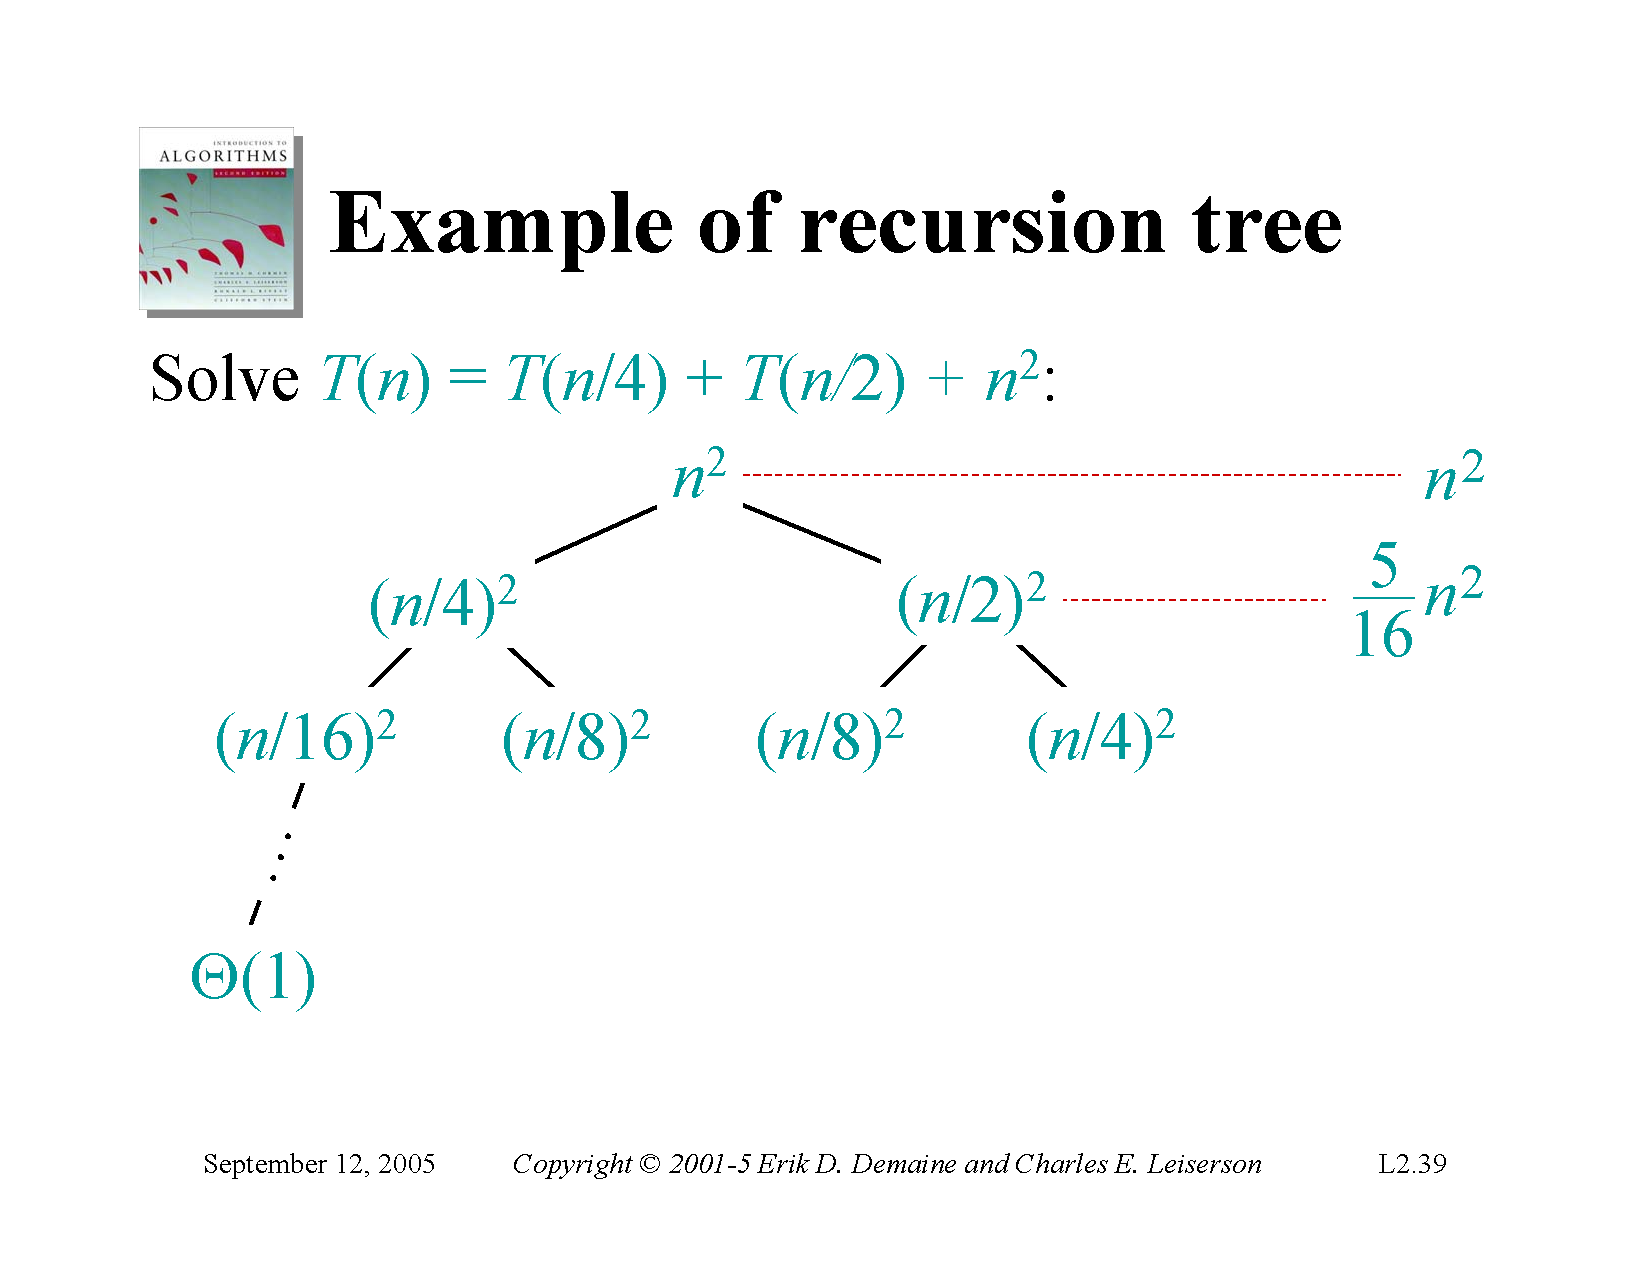
\includegraphics[width=\textwidth, trim={1.10cm 1.20cm 0.30cm 5.75cm}, clip]{pages/lec2_39}
\end{frame}
\begin{frame}{Example of recursion tree}
    Solve $T(n) = T\left(\frac{n}{4}\right) + T\left(\frac{n}{2}\right) + n^2$
    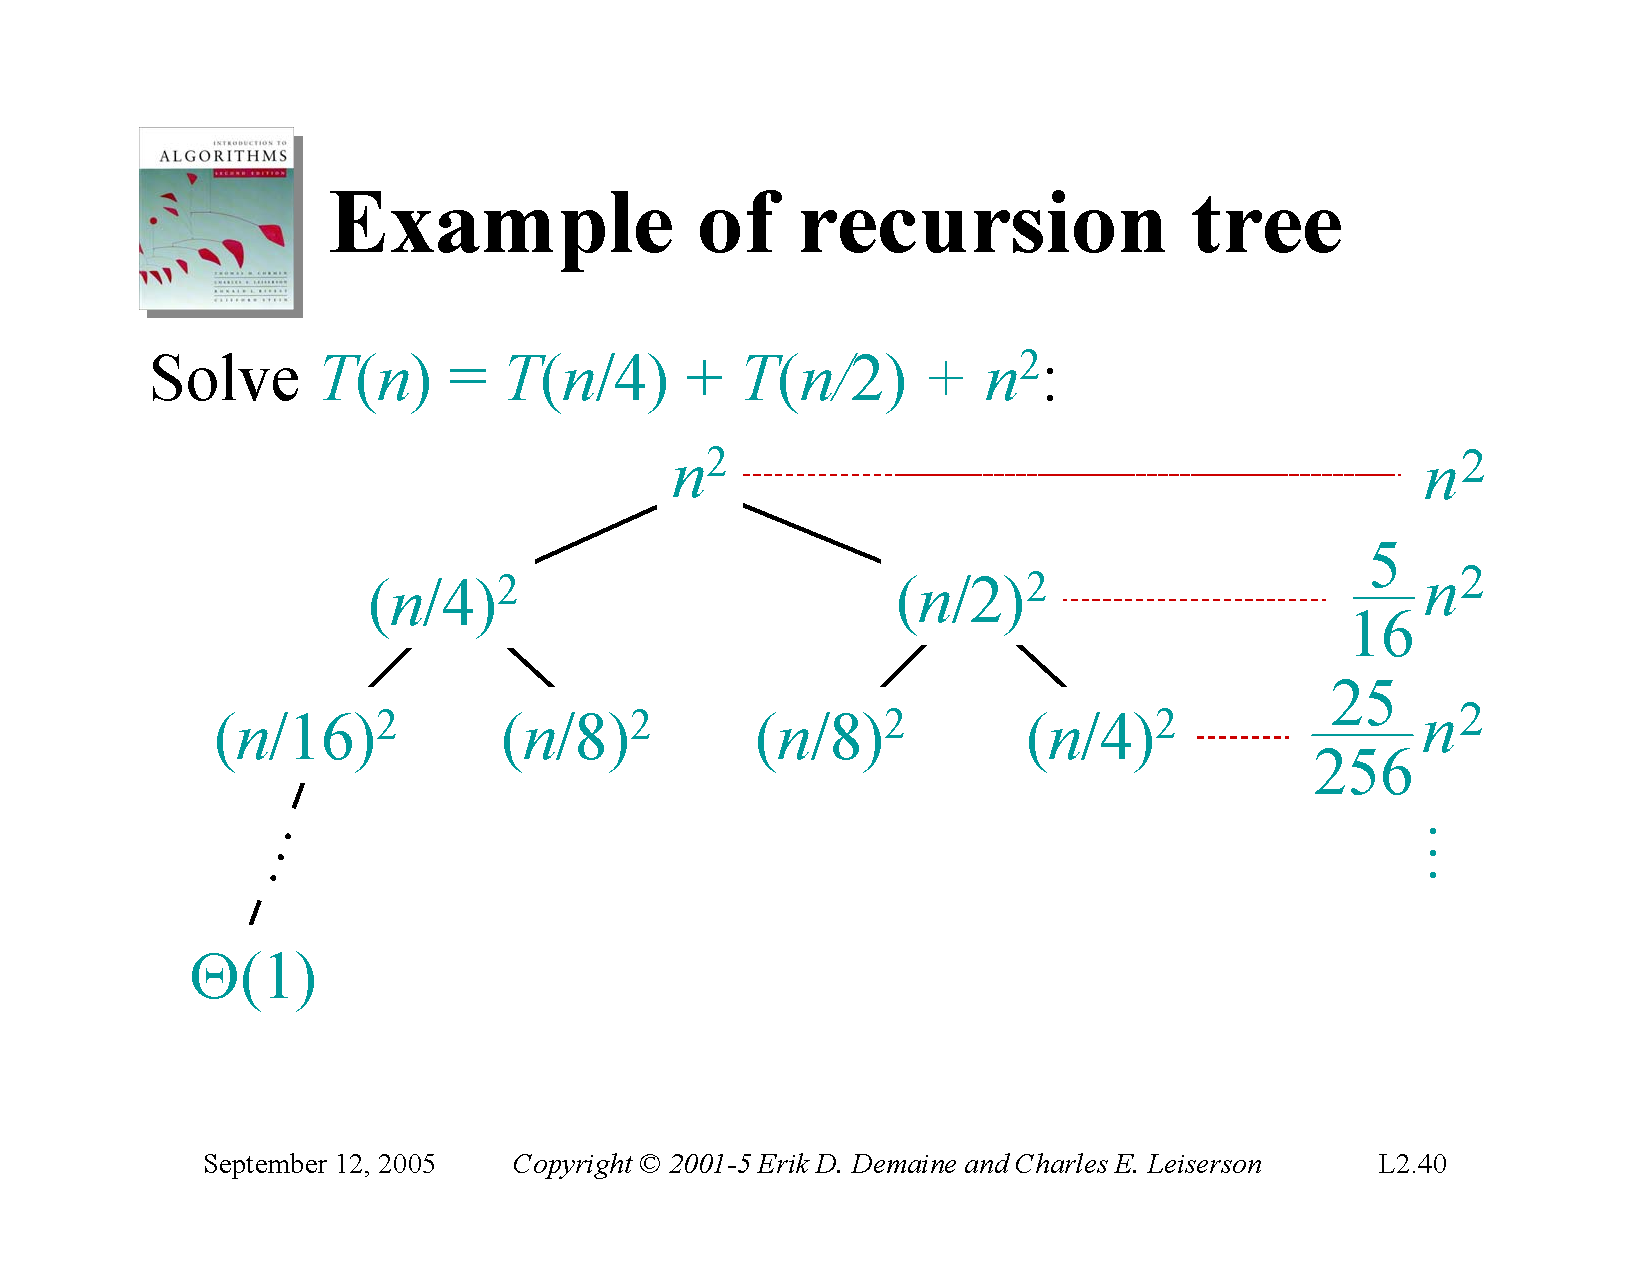
\includegraphics[width=\textwidth, trim={1.10cm 1.20cm 0.30cm 5.75cm}, clip]{pages/lec2_40}
\end{frame}
\begin{frame}{Example of recursion tree}
    Solve $T(n) = T\left(\frac{n}{4}\right) + T\left(\frac{n}{2}\right) + n^2$
    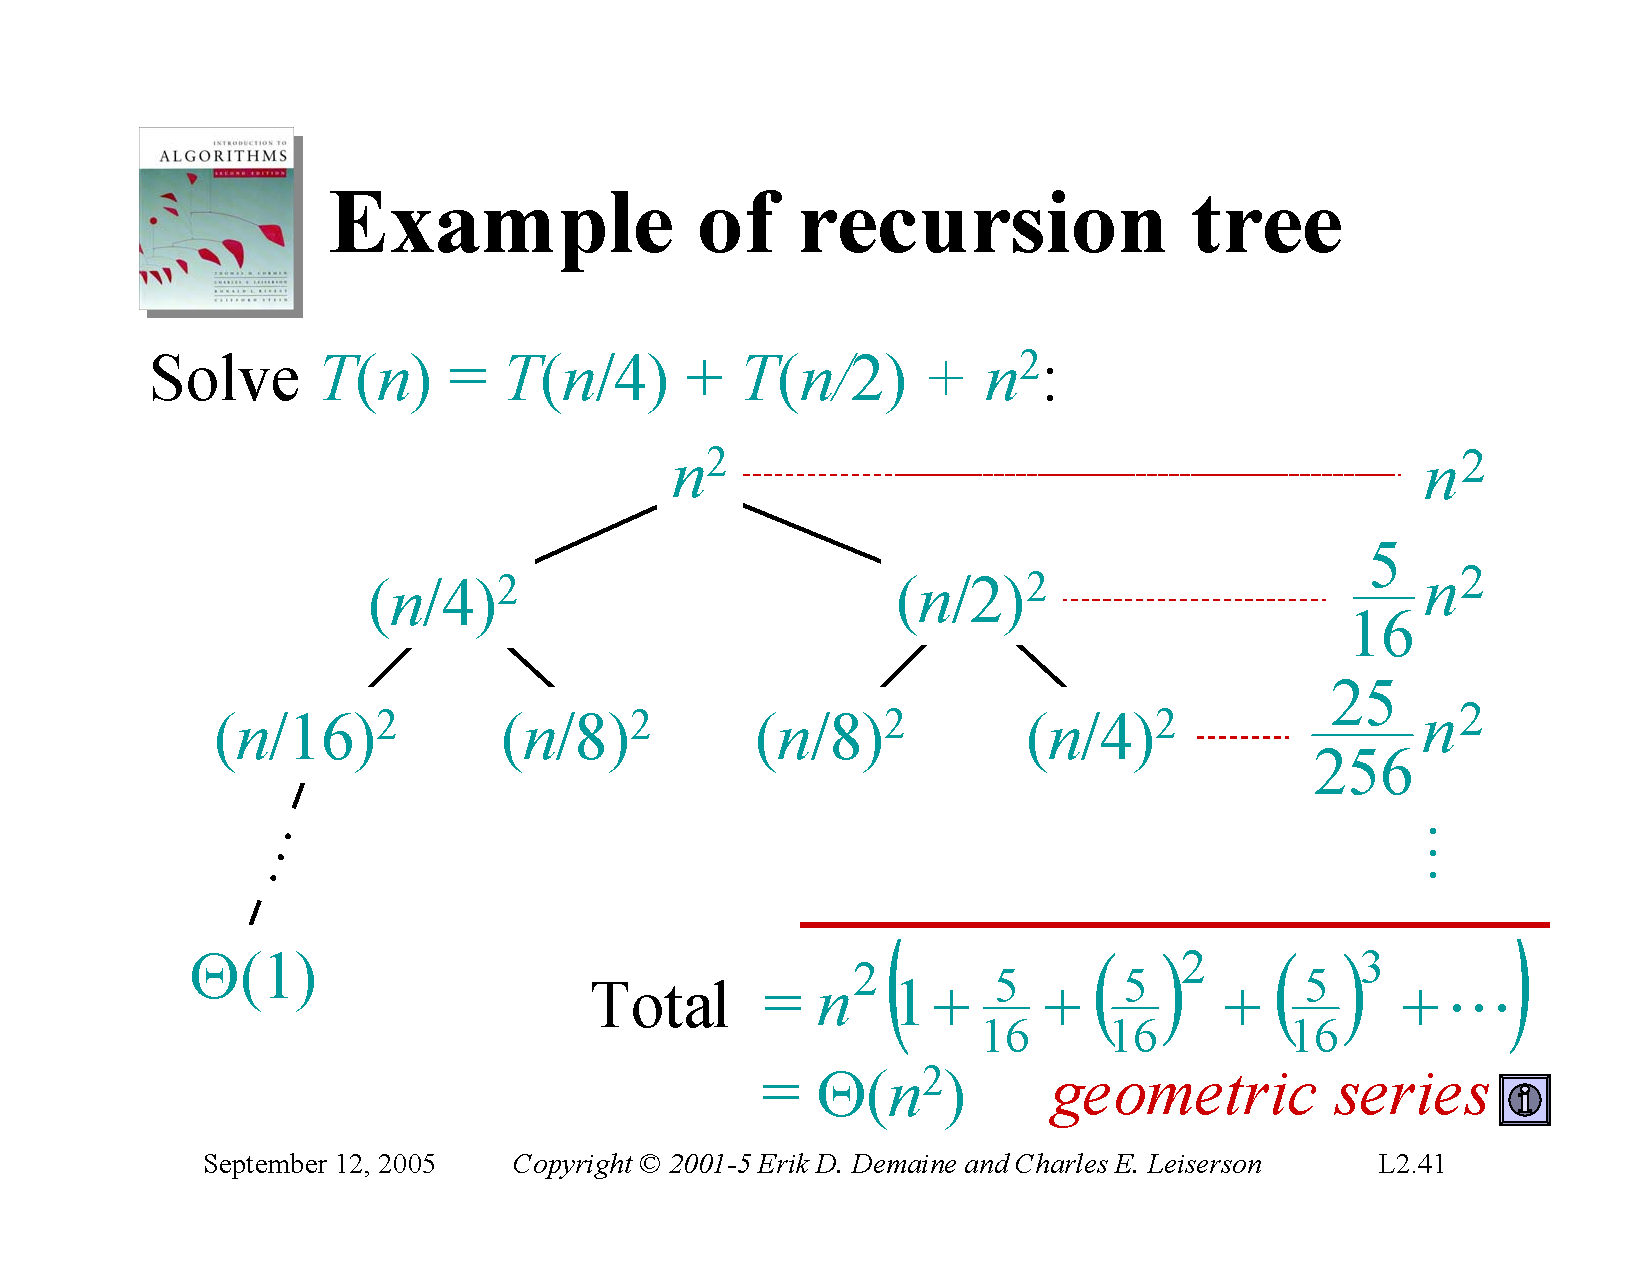
\includegraphics[width=\textwidth, trim={1.10cm 1.20cm 0.30cm 5.75cm}, clip]{pages/lec2_41}
\end{frame}

\subsection{The master method}

\begin{frame}{The master method}
    The master method applies to recurrences of the form:
    $$
        T(n) = aT\left(\frac{n}{b} \right) + f(n) \text{,}
    $$
    \begin{tikzpicture}[remember picture,overlay]
        \draw[red,thick,->]   (2.40, -0.40) to [out=90,in=270](4.85, 0.65);
        \node[] at (2.40, -0.50) {\small You have $a$ subproblems.}; \pause
        \draw[blue,thick,->]  (4.40, -1.30) to [out=90,in=270](5.70, 0.40);
        \node[] at (4.40, -1.50) {\small Each of them is of size $\frac{n}{b}$.}; \pause
        \draw[orange,thick,->](8.40, -2.30) to [out=90,in=270](6.90, 0.60);
        \node[] at (8.40, -2.50) {\small Then you're doing $f(n)$ nonrecursive work.}; \pause
    \end{tikzpicture}
\end{frame}

\begin{frame}{The master method}
    The master method applies to recurrences of the form:
    $$
        T(n) = aT\left(\frac{n}{b} \right) + f(n) \text{,}
    $$
    where $a \geq 1$, $b > 1$, and $f(n)$ is \textit{asymptotically positive}.
\end{frame}

\begin{frame}{The master method}
    The master method applies to recurrences of the form:
    $$
        T(n) = aT\left(\frac{n}{b} \right) + f(n) \text{,}
    $$
    where $a \geq 1$, $b > 1$, and $f(n)$ is \textit{asymptotically positive}.
    \begin{alertblock}{Note}
        \textit{asymptotically positive} means $f(n) > 0$ for $n \geq n_0$.
    \end{alertblock}
\end{frame}

\begin{frame}{Three common cases}
    Compare $f(n)$ with $n^{\log_b a}$: \pause
    \begin{alertblock}{\textbf{Note:}}
        $n^{\log_b a} =$ The number of leaves in the recursion tree.
    \end{alertblock} \pause
    \begin{itemize}
        \item[Case 1] $f(n) < n^{\log_b a}$
        \item[Case 2] $f(n) = n^{\log_b a}$
        \item[Case 3] $f(n) > n^{\log_b a}$
    \end{itemize}


\end{frame}

\begin{frame}{Three common cases}
    Compare $f(n)$ with $n^{\log_b a}$: \pause
    \begin{enumerate}
        \item[1] $f(n) = O\left(n^{\log_b a - \varepsilon} \right)$ for some constant $\varepsilon > 0$.
        \begin{itemize}
            \item $f(n)$ grows polynomially slower than $n^{\log_b a}$ (by an $n^\varepsilon$ factor, polynomially smaller).
            \item \textbf{Solution:} 
                $$
                    T(n) = \Theta(n^{\log_b a}).
                $$
        \end{itemize} \pause
        \item[2] $f(n) = \Theta(n^{\log_b a} \lg^k n)$ for some constant $k \geq 0$.
        \begin{itemize}
            \item $f(n)$ and $n^{\log_b a}$ grow at similar rates, up to poly $\log$ factor.
            \item \textbf{Solution:} 
                $$
                    T(n) = \Theta(n^{\log_b a} \lg^{k+1} n).
                $$
        \end{itemize} \pause
        \item[3] $f(n) = \Omega(n^{\log_b a + \varepsilon})$ for some constant $\varepsilon > 0$.
        \begin{itemize}
            \item $f(n)$ grows polynomially faster than $n^{\log_b a}$ (by an $n^\varepsilon$ factor, polynomially faster), \\
            \textbf{and} $f(n)$ satisfies the \textbf{\textit{regularity condition}} that $af\left(\frac{n}{b}\right) \leq cf(n)$ for some constant $c < 1$. 
            \item \textbf{Solution:} 
                $$
                    T(n) = \Theta(f(n)).
                $$
        \end{itemize}
    \end{enumerate}
\end{frame}

\begin{frame}{Examples}
    \begin{exampleblock}{\textbf{Ex.}}
        \vspace{-8mm}
        \begin{align*}
            & T(n) = 4T\left(\frac{n}{2} \right) + n \\
            & a = 4, b = 2 \implies n^{\log_b a} = n^2 \text{ ; } f(n) = n \text{.} \\
        \end{align*}
    \end{exampleblock}
\end{frame}

\begin{frame}{Examples}
    \begin{exampleblock}{\textbf{Ex.}}
        \vspace{-8mm}
        \begin{align*}
            & T(n) = 4T\left(\frac{n}{2} \right) + n \\
            & a = 4, b = 2 \implies n^{\log_b a} = n^2 \text{ ; } f(n) = n \text{.} \\
            & \text{\textsc{Case 1:}} \\
        \end{align*}
    \end{exampleblock}
\end{frame}

\begin{frame}{Examples}
    \begin{exampleblock}{\textbf{Ex.}}
        \vspace{-8mm}
        \begin{align*}
            & T(n) = 4T\left(\frac{n}{2} \right) + n \\
            & a = 4, b = 2 \implies n^{\log_b a} = n^2 \text{ ; } f(n) = n \text{.} \\
            & \text{\textsc{Case 1:}} f(n) = O(n^{2 - \varepsilon}) \text{ for } \varepsilon = 1 \text{.} \\
        \end{align*}
    \end{exampleblock}
\end{frame}

\begin{frame}{Examples}
    \begin{exampleblock}{\textbf{Ex.}}
        \vspace{-8mm}
        \begin{align*}
            & T(n) = 4T\left(\frac{n}{2} \right) + n \\
            & a = 4, b = 2 \implies n^{\log_b a} = n^2 \text{ ; } f(n) = n \text{.} \\
            & \text{\textsc{Case 1:}} f(n) = O(n^{2 - \varepsilon}) \text{ for } \varepsilon = 1 \text{.} \\
            & \therefore T(n) = \Theta(n^2) \text{.} \\
        \end{align*}
    \end{exampleblock}
\end{frame}

\begin{frame}{Examples}
    \begin{exampleblock}{\textbf{Ex.}}
        \vspace{-8mm}
        \begin{align*}
            & T(n) = 4T\left(\frac{n}{2} \right) + n^2 \\
        \end{align*}
    \end{exampleblock}
\end{frame}

\begin{frame}{Examples}
    \begin{exampleblock}{\textbf{Ex.}}
        \vspace{-8mm}
        \begin{align*}
            & T(n) = 4T\left(\frac{n}{2} \right) + n^2 \\
            & a = 4, b = 2 \implies n^{\log_b a} = n^2 \text{ ; } f(n) = n^2 \text{.} \\
        \end{align*}
    \end{exampleblock}
\end{frame}

\begin{frame}{Examples}
    \begin{exampleblock}{\textbf{Ex.}}
        \vspace{-8mm}
        \begin{align*}
            & T(n) = 4T\left(\frac{n}{2} \right) + n^2 \\
            & a = 4, b = 2 \implies n^{\log_b a} = n^2 \text{ ; } f(n) = n^2 \text{.} \\
            & \text{\textsc{Case 2:}} \\
        \end{align*}
    \end{exampleblock}
\end{frame}

\begin{frame}{Examples}
    \begin{exampleblock}{\textbf{Ex.}}
        \vspace{-8mm}
        \begin{align*}
            & T(n) = 4T\left(\frac{n}{2} \right) + n^2 \\
            & a = 4, b = 2 \implies n^{\log_b a} = n^2 \text{ ; } f(n) = n^2 \text{.} \\
            & \text{\textsc{Case 2:}} f(n) = \Theta(n^2\lg^0n) \text{, that is, } k = 0 \text{.} \\
        \end{align*}
    \end{exampleblock}
\end{frame}

\begin{frame}{Examples}
    \begin{exampleblock}{\textbf{Ex.}}
        \vspace{-8mm}
        \begin{align*}
            & T(n) = 4T\left(\frac{n}{2} \right) + n^2 \\
            & a = 4, b = 2 \implies n^{\log_b a} = n^2 \text{ ; } f(n) = n^2 \text{.} \\
            & \text{\textsc{Case 2:}} f(n) = \Theta(n^2\lg^0n) \text{, that is, } k = 0 \text{.} \\
            & \therefore T(n) = \Theta(n^2 \lg n) \text{.} \\
        \end{align*}
    \end{exampleblock}
\end{frame}

\begin{frame}{Examples}
    \begin{exampleblock}{\textbf{Ex.}}
        \vspace{-8mm}
        \begin{align*}
            & T(n) = 4T\left(\frac{n}{2} \right) + n^3 \\
        \end{align*}
    \end{exampleblock}
\end{frame}

\begin{frame}{Examples}
    \begin{exampleblock}{\textbf{Ex.}}
        \vspace{-8mm}
        \begin{align*}
            & T(n) = 4T\left(\frac{n}{2} \right) + n^3 \\
            & a = 4, b = 2 \implies n^{\log_b a} = n^2 \text{ ; } f(n) = n^3 \text{.} \\
        \end{align*}
    \end{exampleblock}
\end{frame}

\begin{frame}{Examples}
    \begin{exampleblock}{\textbf{Ex.}}
        \vspace{-8mm}
        \begin{align*}
            & T(n) = 4T\left(\frac{n}{2} \right) + n^3 \\
            & a = 4, b = 2 \implies n^{\log_b a} = n^2 \text{ ; } f(n) = n^3 \text{.} \\
            & \text{\textsc{Case 3:}} \\
        \end{align*}
    \end{exampleblock}
\end{frame}

\begin{frame}{Examples}
    \begin{exampleblock}{\textbf{Ex.}}
        \vspace{-8mm}
        \begin{align*}
            & T(n) = 4T\left(\frac{n}{2} \right) + n^3 \\
            & a = 4, b = 2 \implies n^{\log_b a} = n^2 \text{ ; } f(n) = n^3 \text{.} \\
            & \text{\textsc{Case 3:}} f(n) = \Omega(n^{2 + \varepsilon}) \text{ for } \varepsilon = 1 \text{.} \\
        \end{align*}
    \end{exampleblock}
\end{frame}

\begin{frame}{Examples}
    \begin{exampleblock}{\textbf{Ex.}}
        \vspace{-8mm}
        \begin{align*}
            & T(n) = 4T\left(\frac{n}{2} \right) + n^3 \\
            & a = 4, b = 2 \implies n^{\log_b a} = n^2 \text{ ; } f(n) = n^3 \text{.} \\
            & \text{\textsc{Case 3:}} f(n) = \Omega(n^{2 + \varepsilon}) \text{ for } \varepsilon = 1 \text{.} \\
            & \text{\textbf{and} } 4\left(\frac{n}{2} \right)^3 \leq cn^3 \text{ (reg. cond.) for } c = \frac{1}{2} \text{.} \\
        \end{align*}
    \end{exampleblock}
\end{frame}

\begin{frame}{Examples}
    \begin{exampleblock}{\textbf{Ex.}}
        \vspace{-8mm}
        \begin{align*}
            & T(n) = 4T\left(\frac{n}{2} \right) + n^3 \\
            & a = 4, b = 2 \implies n^{\log_b a} = n^2 \text{ ; } f(n) = n^3 \text{.} \\
            & \text{\textsc{Case 3:}} f(n) = \Omega(n^{2 + \varepsilon}) \text{ for } \varepsilon = 1 \text{.} \\
            & \text{\textbf{and} } 4\left(\frac{n}{2} \right)^3 \leq cn^3 \text{ (reg. cond.) for } c = \frac{1}{2} \text{.} \\
            & \therefore T(n) = \Theta(n^3) \text{.} \\
        \end{align*}
    \end{exampleblock}
\end{frame}

\begin{frame}{Examples}
    \begin{exampleblock}{\textbf{Ex.}}
        \vspace{-8mm}
        \begin{align*}
            & T(n) = 4T\left(\frac{n}{2} \right) + \frac{n^2}{\lg n} \\
        \end{align*}
    \end{exampleblock}
\end{frame}

\begin{frame}{Examples}
    \begin{exampleblock}{\textbf{Ex.}}
        \vspace{-8mm}
        \begin{align*}
            & T(n) = 4T\left(\frac{n}{2} \right) + \frac{n^2}{\lg n} \\
            & a = 4, b = 2 \implies n^{\log_b a} = n^2 \text{ ; } f(n) = \frac{n^2}{\lg n} \text{.} \\
        \end{align*}
    \end{exampleblock}
\end{frame}

\begin{frame}{Examples}
    \begin{exampleblock}{\textbf{Ex.}}
        \vspace{-8mm}
        \begin{align*}
            & T(n) = 4T\left(\frac{n}{2} \right) + \frac{n^2}{\lg n} \\
            & a = 4, b = 2 \implies n^{\log_b a} = n^2 \text{ ; } f(n) = \frac{n^2}{\lg n} \text{.} \\
        \end{align*}
        \vspace{-10mm}
        \small
        \begin{itemize}
            \item $f(n) = \frac{n^2}{\lg n}$. Have $f(n) = o(n)$, so that $f(n)$ grows more slowly than $n$, it doesn’t grow polynomially slower.
            \item In terms of the master theorem, have $f(n) = n^2\lg^{-1} n$, so that $k = -1$.
            \item Master theorem holds only for $k \geq 0$, so case 2 does not apply.
            \item Master method does not apply.
        \end{itemize}
    \end{exampleblock}
\end{frame}

\begin{frame}{Intuition behind of master theorem}
    \textit{Recursion tree:}\\
    \vspace{5mm}
    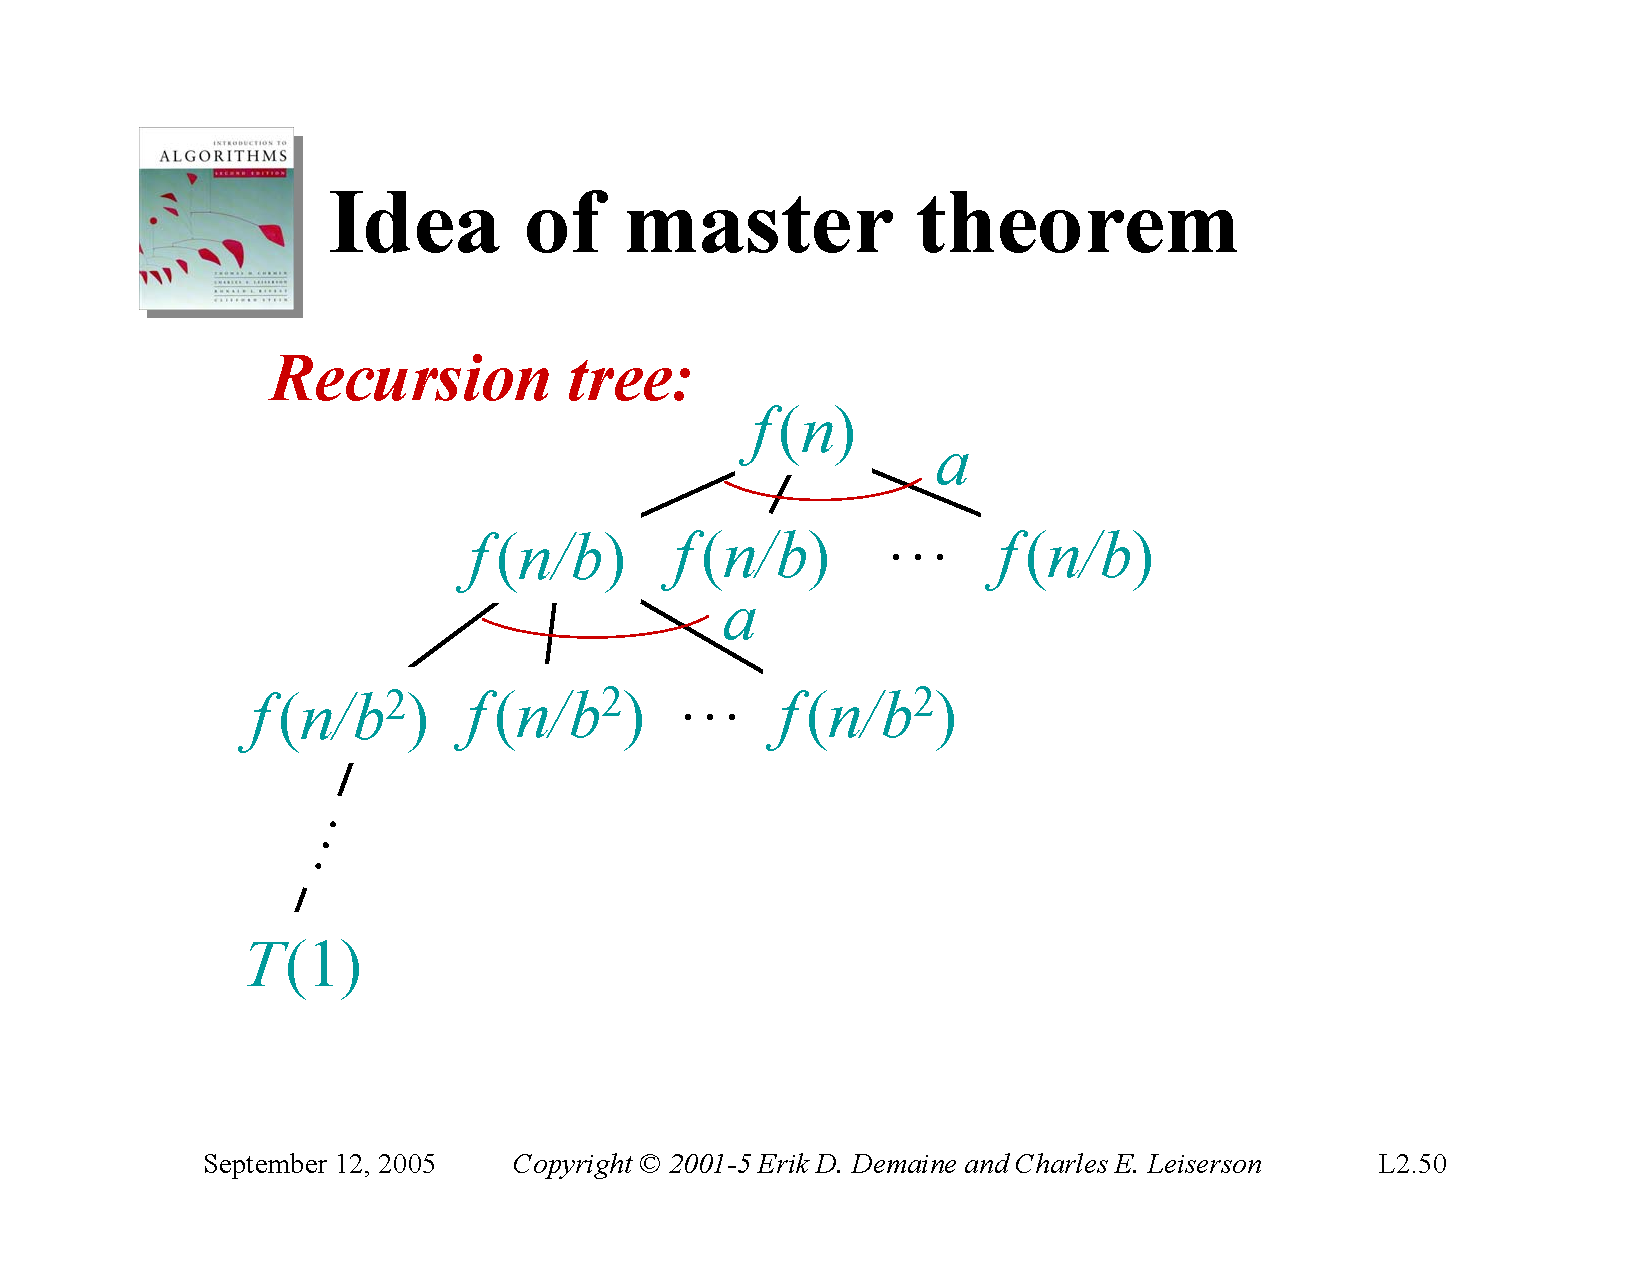
\includegraphics[width=\textwidth, trim={1.10cm 1.20cm 0.30cm 5.50cm}, clip]{pages/lec2_50}
\end{frame}
\begin{frame}{Intuition behind of master theorem}
    \textit{Recursion tree:}\\
    \vspace{5mm}
    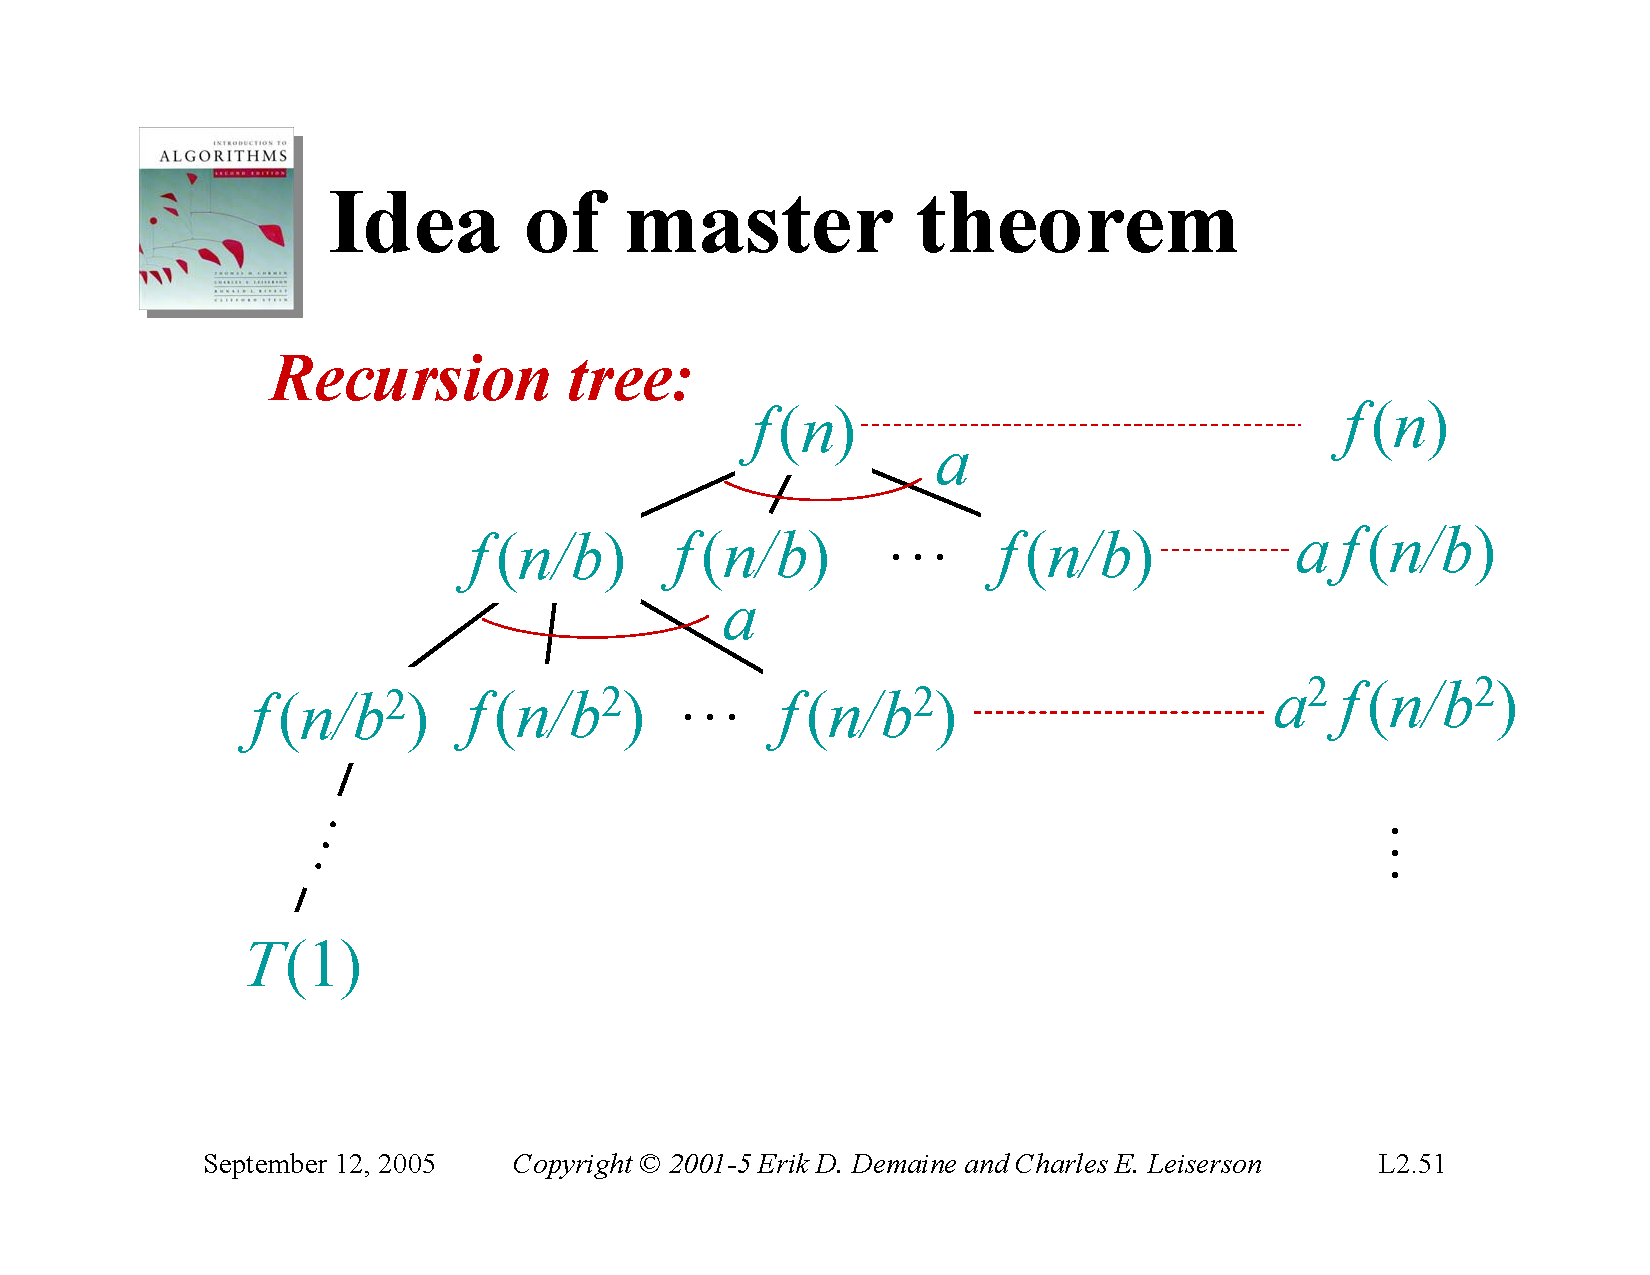
\includegraphics[width=\textwidth, trim={1.10cm 1.20cm 0.30cm 5.50cm}, clip]{pages/lec2_51}
\end{frame}
\begin{frame}{Intuition behind of master theorem}
    \textit{Recursion tree:}\\
    \vspace{5mm}
    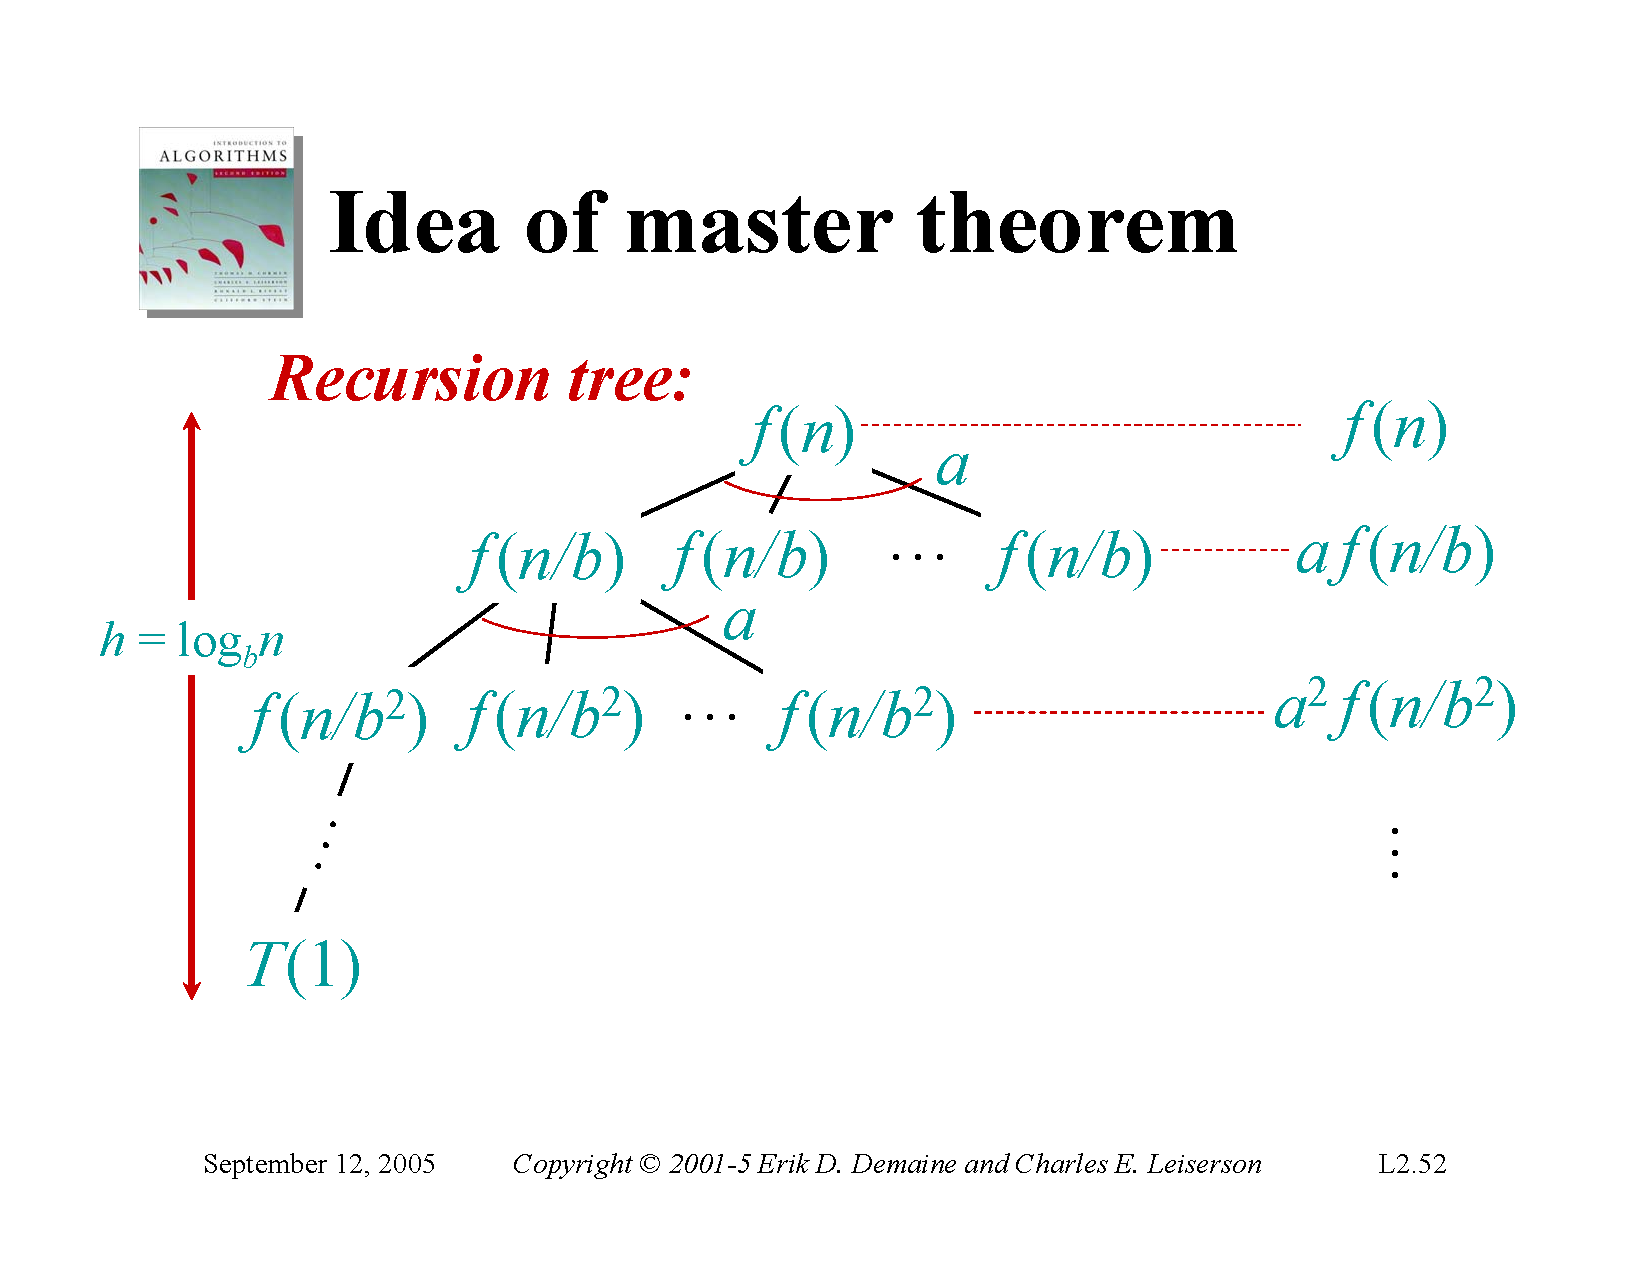
\includegraphics[width=\textwidth, trim={1.10cm 1.20cm 0.30cm 5.50cm}, clip]{pages/lec2_52}
\end{frame}
\begin{frame}{Intuition behind of master theorem}
    \textit{Recursion tree:}\\
    \vspace{5mm}
    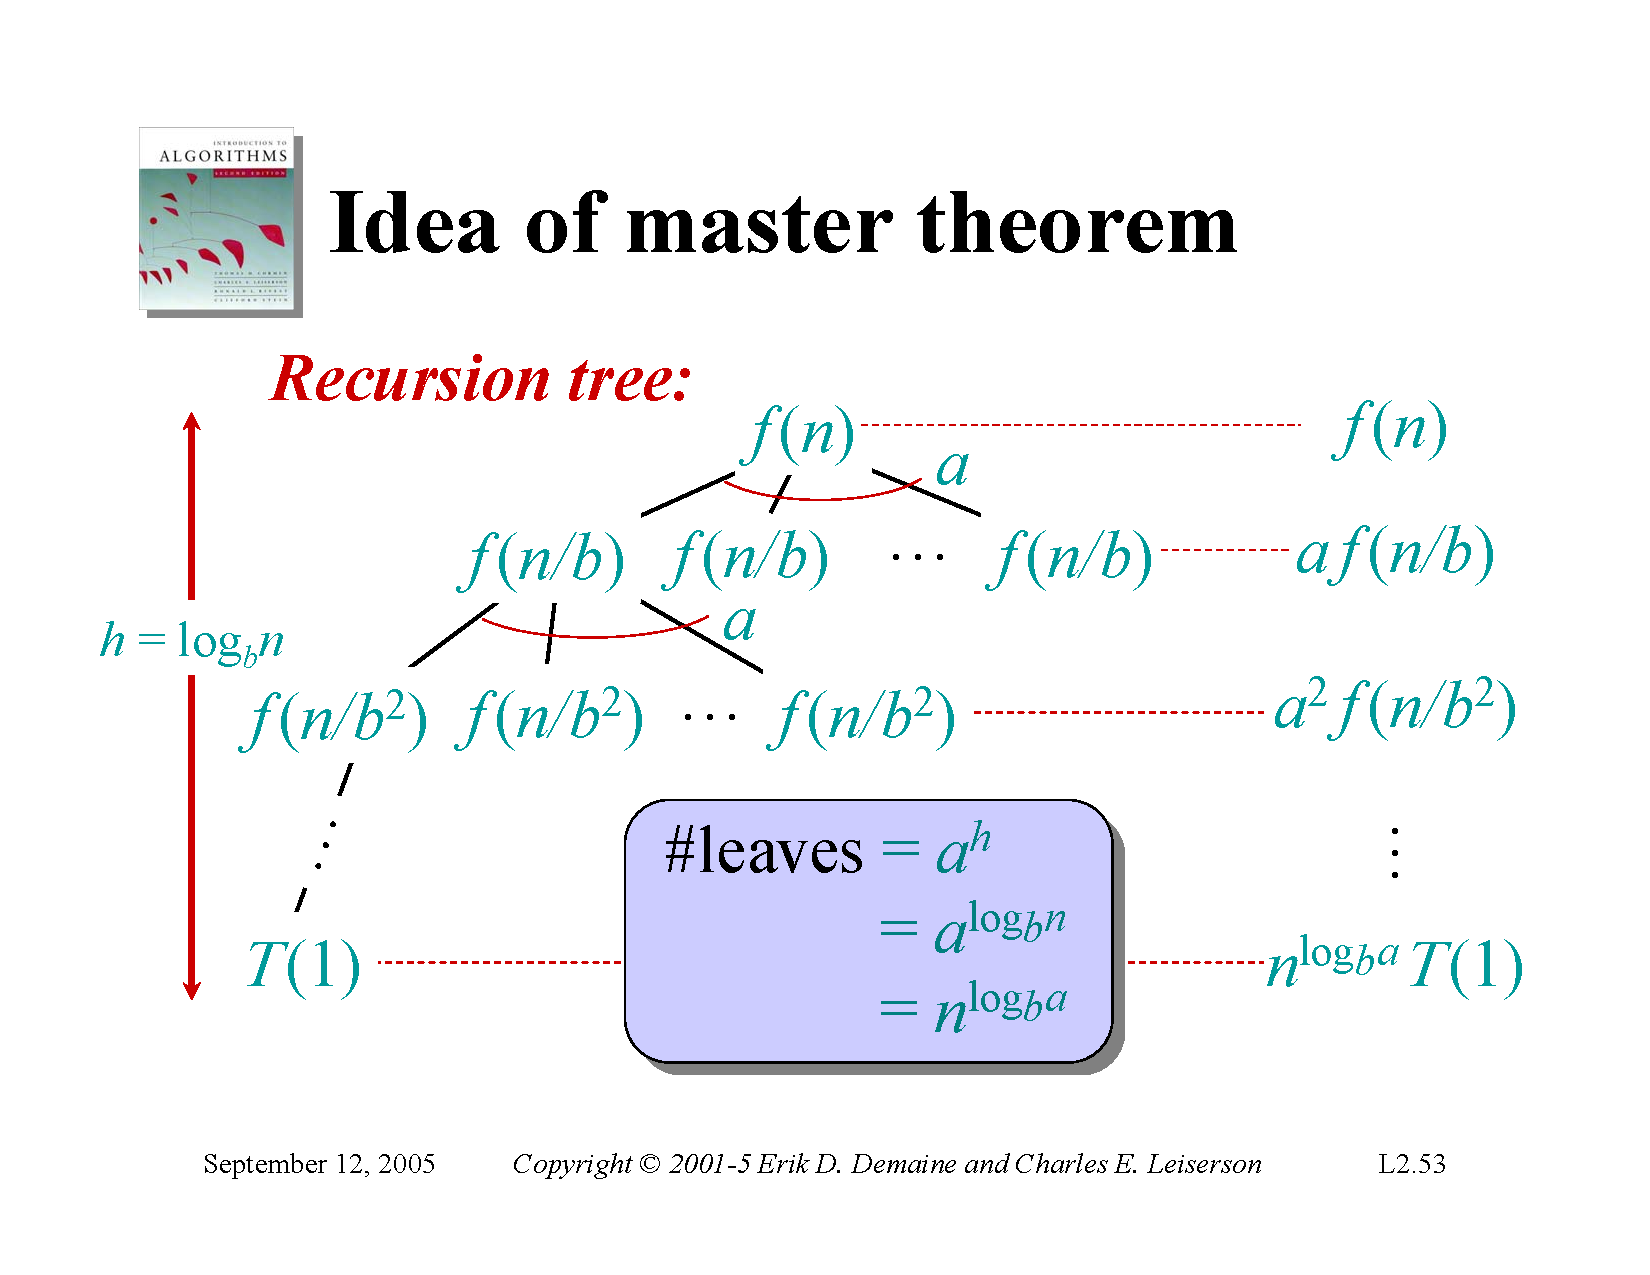
\includegraphics[width=\textwidth, trim={1.10cm 1.20cm 0.30cm 5.50cm}, clip]{pages/lec2_53}
\end{frame}
\begin{frame}{Intuition behind of master theorem}
    \textit{Recursion tree:}\\
    \vspace{5mm}
    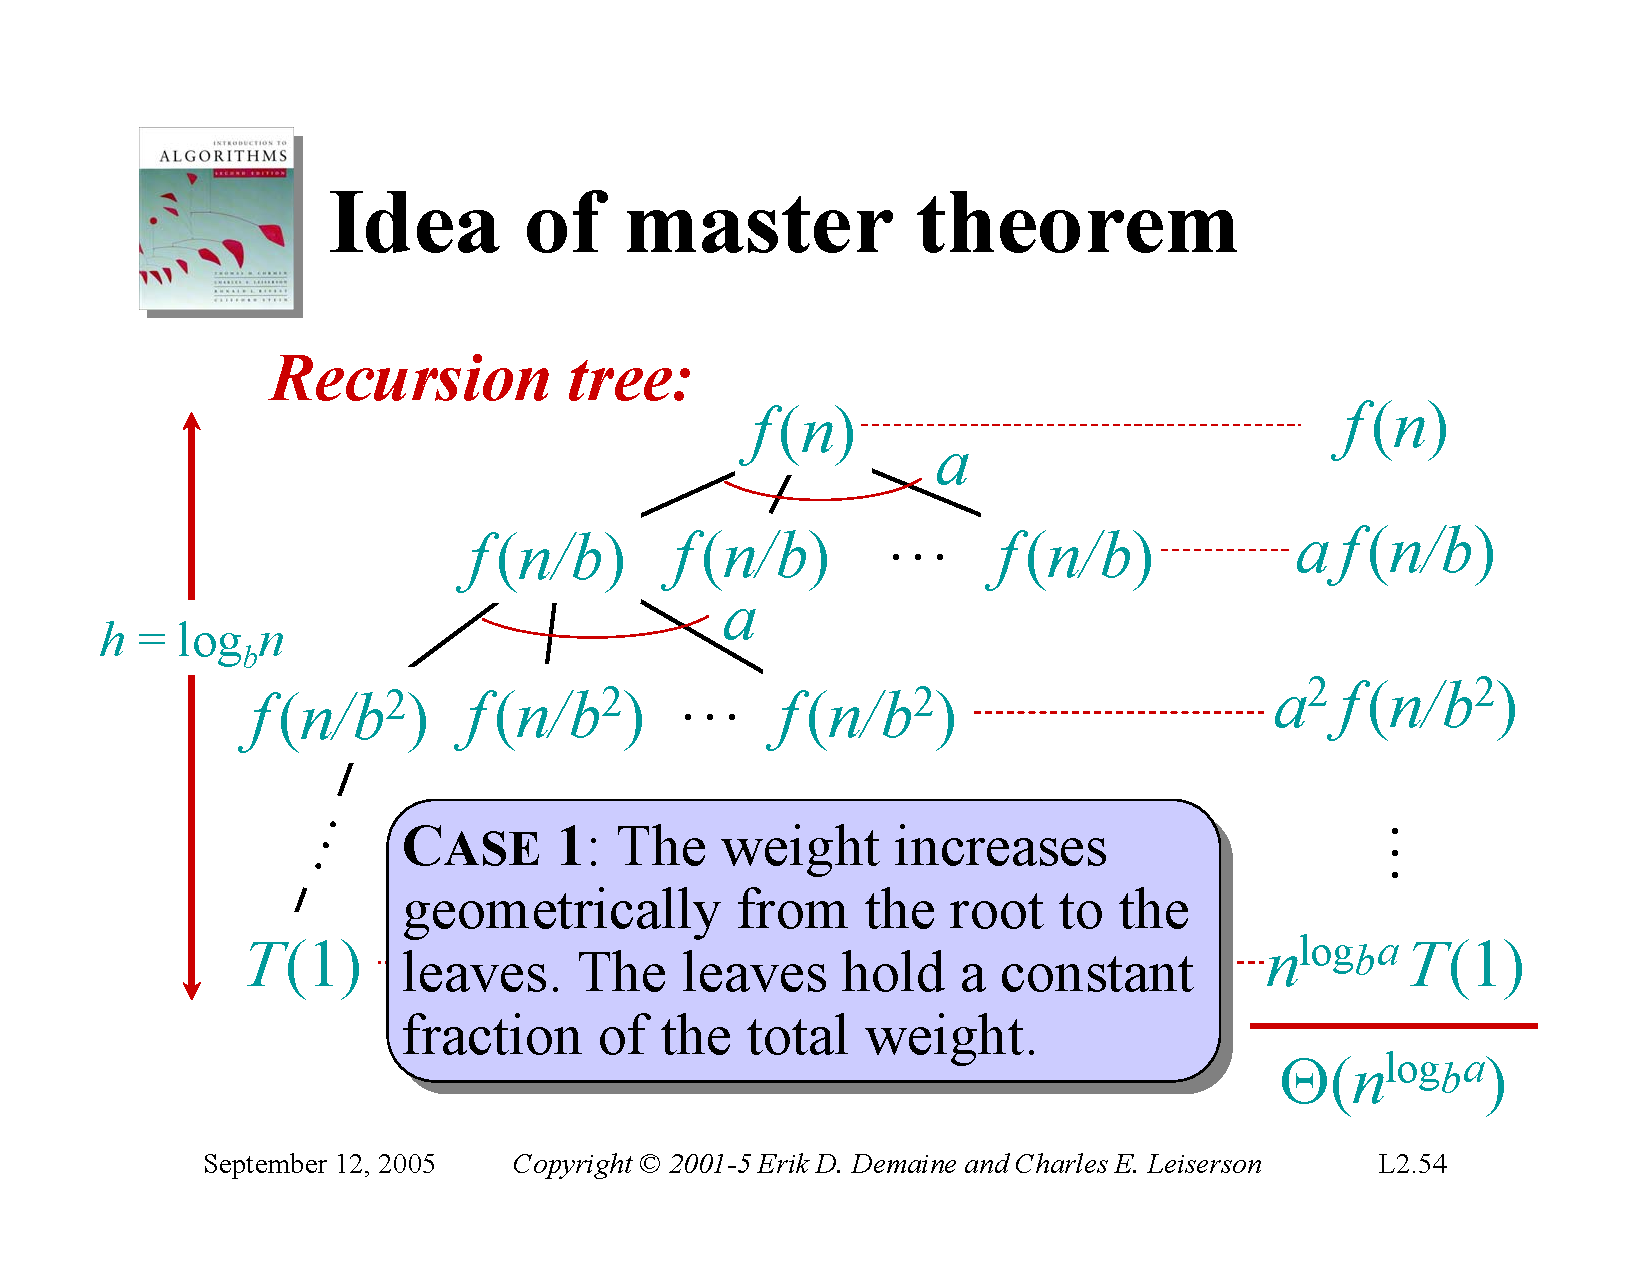
\includegraphics[width=\textwidth, trim={1.10cm 1.20cm 0.30cm 5.50cm}, clip]{pages/lec2_54}
\end{frame}
\begin{frame}{Intuition behind of master theorem}
    \textit{Recursion tree:}\\
    \vspace{5mm}
    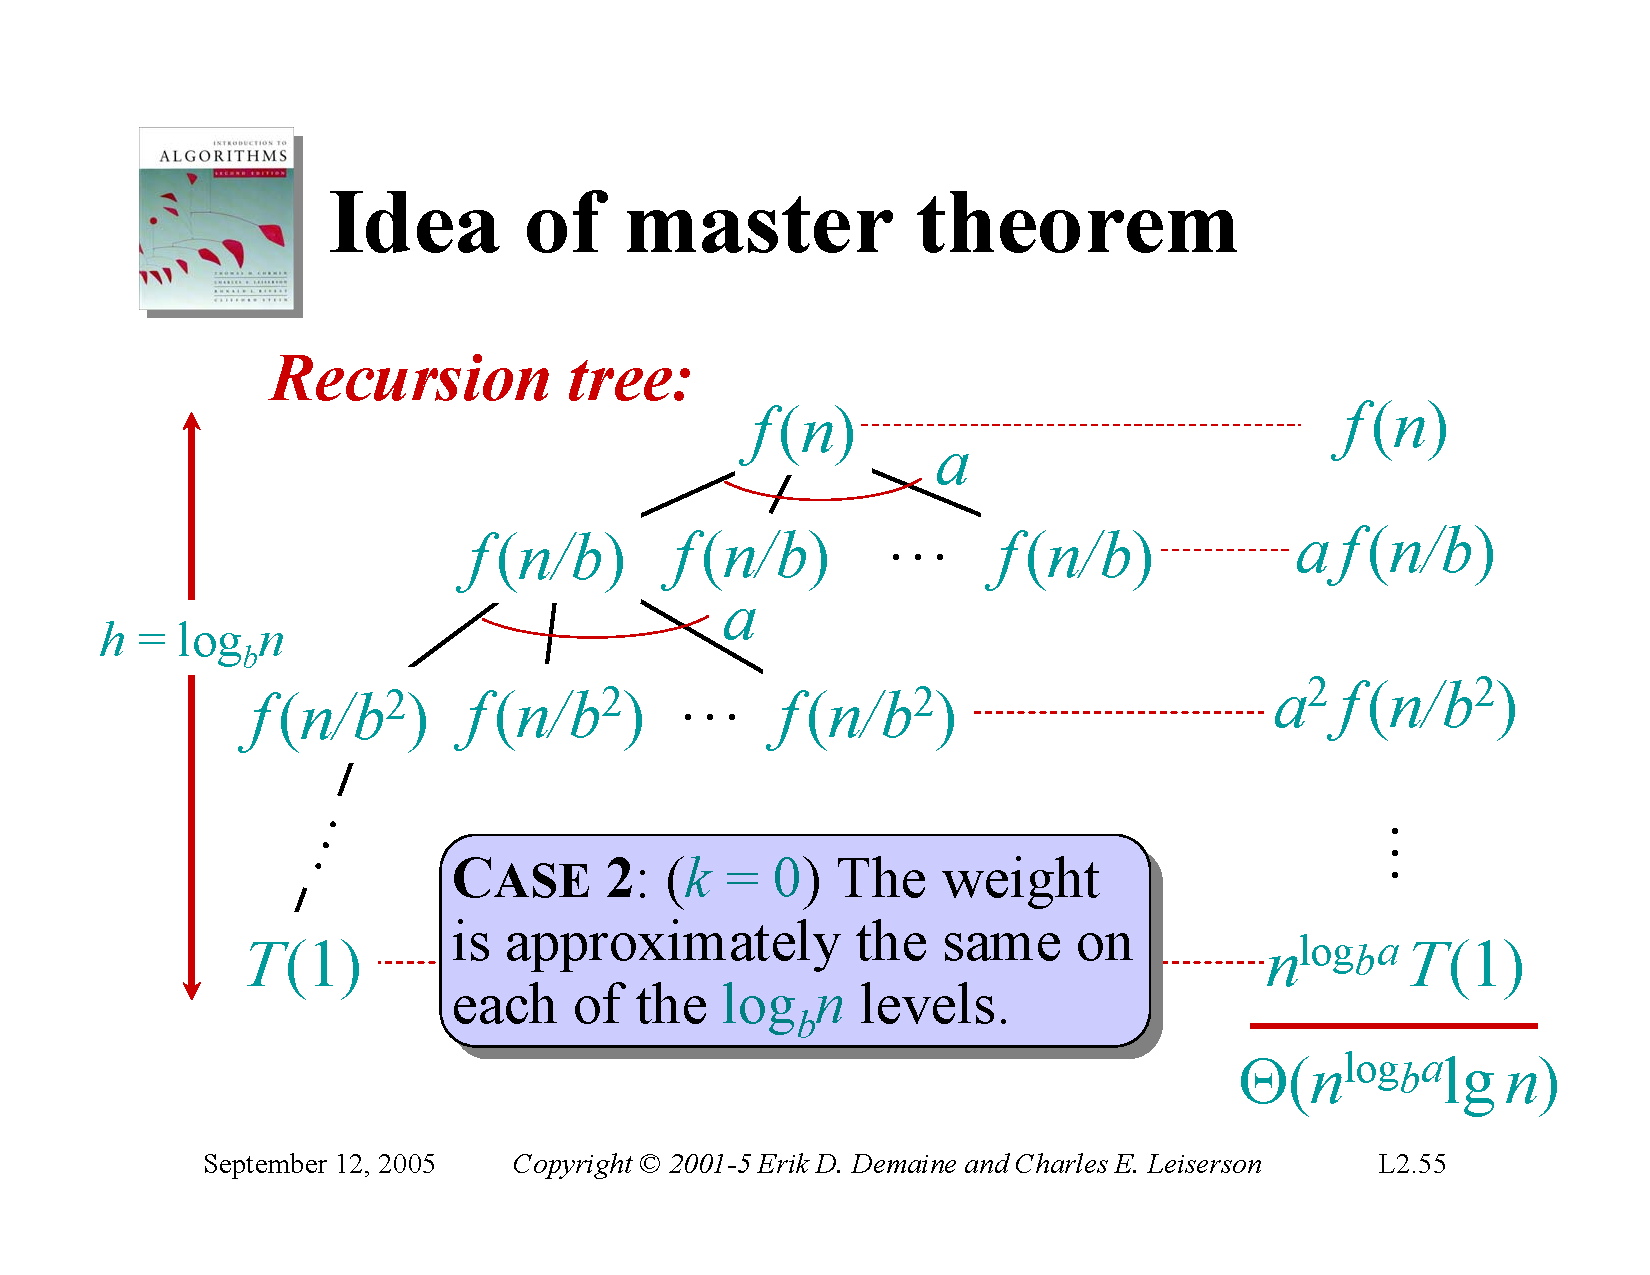
\includegraphics[width=\textwidth, trim={1.10cm 1.20cm 0.30cm 5.50cm}, clip]{pages/lec2_55}
\end{frame}
\begin{frame}{Intuition behind of master theorem}
    \textit{Recursion tree:}\\
    \vspace{5mm}
    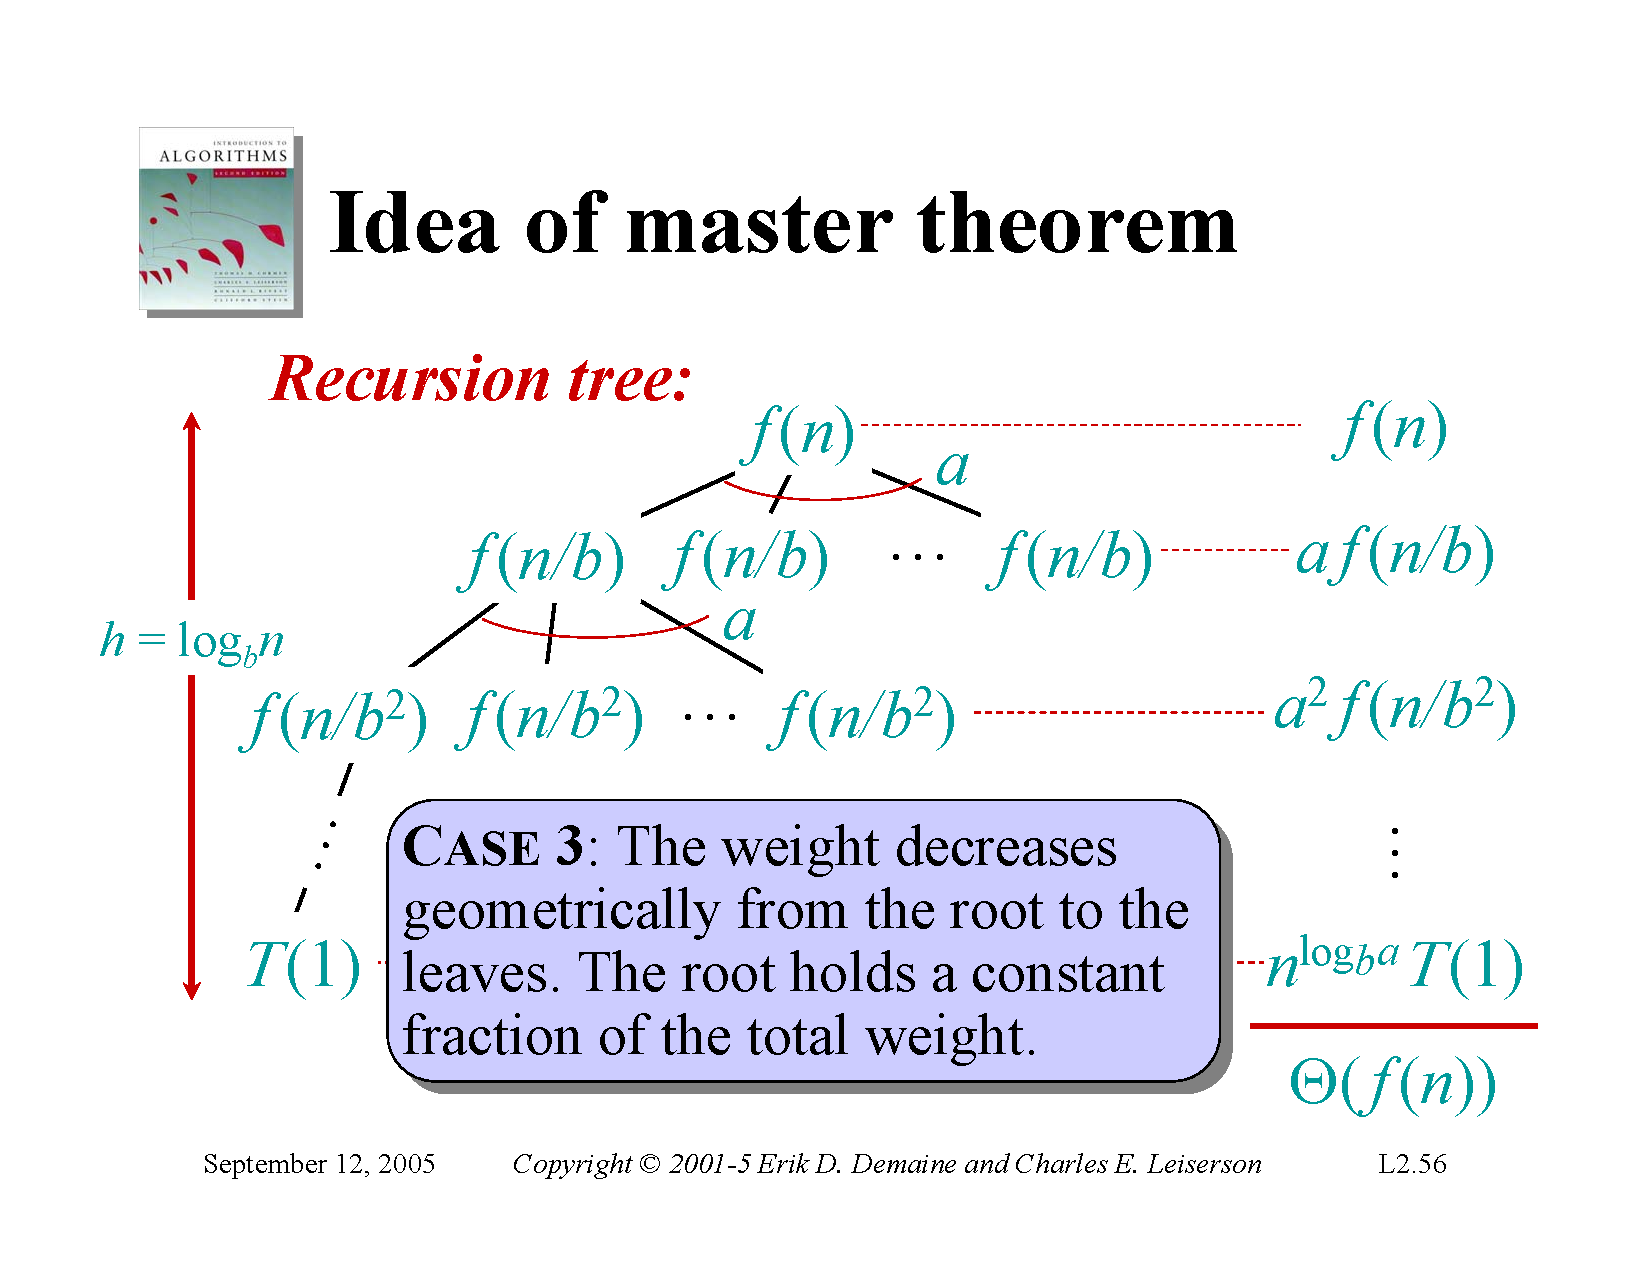
\includegraphics[width=\textwidth, trim={1.10cm 1.20cm 0.30cm 5.50cm}, clip]{pages/lec2_56}
\end{frame}

\begin{frame}{Appendix: geometric series}
    $$
        1 + x + x^2 + \cdots + x^n = \frac{1 - x^{n + a}}{1 - x} \text{ for } x \neq 1
    $$
    
    $$
        1 + x + x^2 + \cdots = \frac{1}{1 - x} \text{ for } |x| < 1
    $$
\end{frame}

\begin{frame}{}
    \centering
    \Huge End of Lecture 2.
\end{frame}

\section*{Takeaways}

\begin{frame}{TDT5FTOTTC}
    \centering
    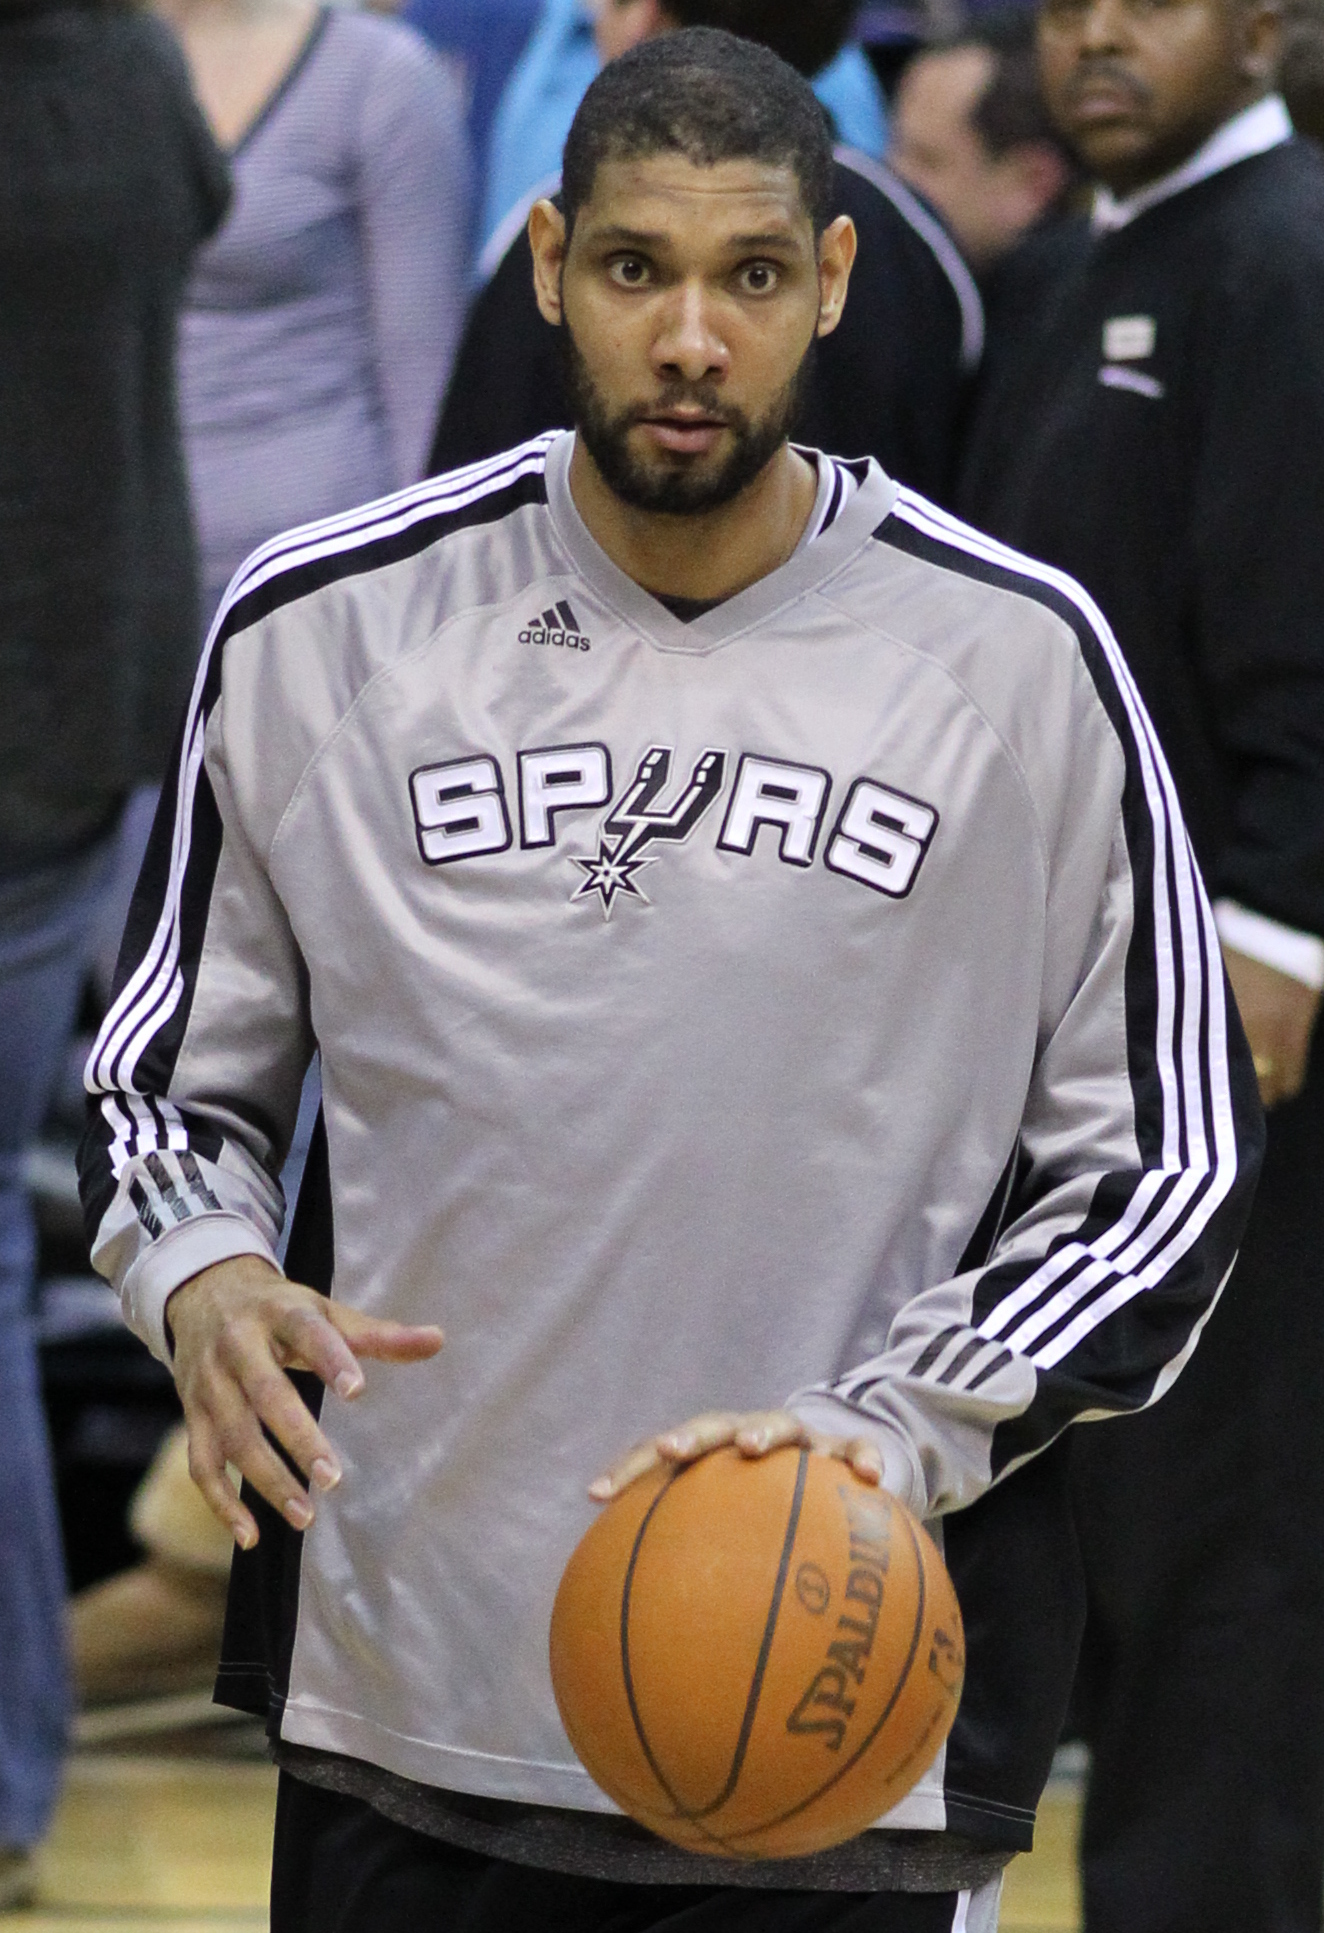
\includegraphics[width=0.45\textwidth]{figures/td.jpg}\\
    \href{https://en.wikipedia.org/wiki/Tim_Duncan}{Tim Duncan in Wikipedia.}
\end{frame}

% Tim Duncan's Top 5 Fundamental Takeaways of the Today's Class
\begin{frame}{TDT5FTOTTC}
    \centering
    
\includegraphics[width=0.75\textwidth]{figures/tim.png}
\end{frame}

\begin{frame}{Top 5 Fundamental Takeaways}
    \small
    \begin{enumerate} \pause
        \item[5] \textbf{Solving Recurrences:} Common methods to solve recurrences include substitution, recursion trees, and the master theorem, each providing different approaches to analyze recursive complexity. \pause

        \item[4] \textbf{Tightening Bounds Using Substitution:} Strengthening inductive hypotheses by subtracting lower-order terms helps refine bounds when standard methods provide loose approximations. \pause

        \item[3] \textbf{Recursion Tree Intuition:} A recursion tree models the breakdown of recursive calls, where the total complexity is derived by summing work across all levels. \pause

        \item[2] \textbf{Master Theorem Cases:} The master theorem classifies recurrences into three cases based on how $f(n)$ compares to $n^{log_b(a)}$, determining whether recursion, work per level, or additional growth dominates. \pause

        \item[1] \textbf{$O$, $\Omega$, and $\Theta$} notations describe upper, lower, and tight bounds on algorithm growth, while $o$ and $\omega$ represent strict bounds. \pause

    \end{enumerate}
\end{frame}

\begin{frame}{Introduction to Algorithms}
    \centering
    
\includegraphics[width=0.45\textwidth]{figures/book_cover.jpg} \\
    \vspace{5mm}
    {
        \tiny
        Content has been extracted from \textit{Introduction to Algorithms}, Fourth Edition, by Cormen, Leiserson, Rivest, and Stein. MIT Press. 2022.\\
        Visit \url{https://mitpress.mit.edu/9780262046305/introduction-to-algorithms/}.\\
        Original slides from \textit{Introduction to Algorithms 6.046J/18.401J}, Fall 2005 Class by Prof. Charles Leiserson and Prof. Erik Demaine. MIT OpenCourseWare Initiative available at \url{https://ocw.mit.edu/courses/6-046j-introduction-to-algorithms-sma-5503-fall-2005/}.\\
    }
\end{frame}

\end{document}
